\chapter{\label{par_est}Parameter estimation using SOAP}
%%%%%%%%%%%%
%%%%%%%%%%%%
%%%%%%%%%%%%
%%%%%

Throughout chapters \ref{soap} and \ref{machine} we~\chris{have} developed
techniques which~\chris{that?} could identify whether a potential \gls{CW}
signal is present within a small frequency band of width $0.1$ Hz, and then
return the frequency track that the signal is most likely to follow.  This
provides frequency bands in which a signal could be present, which is useful
for all-sky searches as it can limit the parameter space and therefore
computational time for deeper searches such as those described in
Sec.~\ref{searchcw:search:targeted}.  However, this only limits the parameter
space in frequency to a smaller frequency band, where there is still a large
parameter space which needs to be searched.  If the Viterbi track returned by
SOAP in chapter \ref{soap} follows the frequency evolution of a \gls{CW}
source, then this track contains information on the sky position and frequency
evolution of the \gls{CW}.  If one could extract this information then the size
of the parameter space for more sensitive searches such as
Einstein@Home~\chris{maybe list a LIGO follow-up rather than EatH?} could be
reduced, decreasing their computational cost.

In this chapter I will outline a Bayesian method which~\chris{the rule for
using "which" rather than "that" is that when you use "which" the sentence
should still make sense if you remove it. If it sounds wrong when you remove
the word then "that" is the correct one to use. In this case, "that" is what
you should use.} uses the output Viterbi tracks of the SOAP search in Chapter
~\ref{soap} to return some~\chris{a subset of?} astrophysical parameters of a
source.  Section~\ref{par_est:freq} will outline the model of the frequency
evolution of a \gls{CW} from a source with a slowly varying frequency,
Sec.~\ref{par_est:bayes} will outline the Bayesian model for this analysis and
Sec.~\ref{par_est:results} will show the results from testing on simulated
signals.

%%%%
%%%%
\section{\label{par_est:freq}\gls{CW} source frequency evolution}
%%%%
%%%%

The SOAP search returns a frequency track known as the Viterbi track, if this
track follows the frequency of a \gls{CW} source, then the frequency evolution
contains information of the sky position ($\alpha, \delta$), the frequency of
the source $f$ and its derivative $\dot{f}$, where we ignore higher order
frequency derivatives.  From the Viterbi track, we should then be able to
extract this information as we have a model for the phase evolution (and
therefore frequency evolution) of the source described in
Eq.~\ref{searchcw:model:phase} in Sec.~\ref{searchcw:model}.  To relate this
phase evolution to the sky position parameters, we can look closer at
Eq.~\ref{searchcw:model:ssbtime}, where we describe the shift in arrival time
due to the earths motion.~\chris{I have no comments on this paragraph!} 

The second term in Eq.~\ref{searchcw:model:ssbtime} describes the Doppler shift
due to the earth's orbit and rotation.  Where the $\bm{r}$ is the position of
the detector and $\bm{n}$ is a unit vector in the direction of the source.  As
in \citep{schutz1998DataAnalysis}, we use the coordinate frame in the \gls{SSB}
where the $z$ axis is perpendicular to the ecliptic and the $x$ axis is
parallel to the celestial sphere.  In this frame the unit vector pointing
towards the star~\chris{source?} can be written as
%
\begin{equation}
    \label{par_est:freq:unit}
    \bm{n} = 
    \left(
    \begin{matrix}
        1 & 0 & 0  \\
        0 & \cos \epsilon & \sin \epsilon \\
        0 & -\sin \epsilon & \cos \epsilon \\
    \end{matrix} \right)
    \left(
    \begin{matrix}
        \cos(\alpha)\cos(\delta)  \\
        \sin(\alpha)\cos(\delta) \\
        \sin(\delta) \\
    \end{matrix} \right),
\end{equation}
%
where $\alpha$ and $\delta$ are the right ascension and declination (sky
position) of the source and $\epsilon$ is the angle between the ecliptic and
the earth's equator.  The first matrix in Eq.~\ref{par_est:freq:unit} describes
a rotation from the celestial frame where $\alpha$ and $\delta$ are measured to
the ecliptic frame~\chris{grammar - reads funny}.  The second matrix~\chris{not
a matric, a vector} transforms the sky position parameters to their component
$x,y,z$ coordinates.

The position vector of the earth~\chris{I hope you mean detector not earth},
$\bm{r}$ in Eq.~\ref{searchcw:model:ssbtime}, at a time $t$ can be split into
the addition of~\chris{into the addition of?  Just split into} two components,
the position due to the orbit of the earth and position due to the rotation of
the earth~\chris{of the detector - see comment at the start of the paragraph}.
If we assume the orbit is circular, then the position of the earth in its orbit
is described in Cartesian coordinates as
%
\begin{equation}
    \bm{r}_{\rm{orb}} = R_{\mathrm{O}}
    \left(
    \begin{matrix}
        \cos{\left( \Omega_{\mathrm{O}} t + \phi_{O}  \right)}  \\
        \sin{\left( \Omega_{\mathrm{O}} t + \phi_{O}  \right)} \\
        0 \\
    \end{matrix} \right),
\end{equation}
%
where $R_{\mathrm{O}}$ is the radius of the earth's orbit (1 AU),
$\Omega_{\mathrm{O}}$ is the angular frequency of the earth's orbit
$2\pi/T_{\mathrm{O}}$, where $T_{\mathrm{O}}$ is one year and $\phi_{O}$ is
some phase which defines the position of the earth in its orbital motion.  The
position due to the rotation of the earth can then be described by 
%
\begin{equation}
    \bm{r}_{\rm{rot}} = R_{\mathrm{R}}
    \left(
    \begin{matrix}
        1 & 0 & 0  \\
        0 & \cos \epsilon & \sin \epsilon \\
        0 & -\sin \epsilon & \cos \epsilon \\
    \end{matrix} \right)
    \left(
    \begin{matrix}
        \cos{(\lambda)}\cos{\left( \Omega_{\mathrm{R}} t + \phi_{R}  \right)}  \\
        \cos{(\lambda)}\sin{\left( \Omega_{\mathrm{R}} t + \phi_{R}  \right)} \\
        \sin{(\lambda)} \\
    \end{matrix} \right),
\end{equation}
%
where $R_{\mathrm{R}}$ is the radius of the earth, $\Omega_{\mathrm{R}}$ is the
angular frequency of the earth's rotation $2\pi/T_{\mathrm{R}}$, where
$T_{\mathrm{R}}$ is one day, $\phi_{O}$ is some phase which defines the
position of the earth in its rotational motion and $\lambda$ is the latitude of
the detectors site~\chris{I'm concerned that the arbitary undefined orbital
phase and rotation phase are determined by the detector longitude and the start
time of the observation. Do you address this further on?}. These two components
can then be added to find~\chris{define?} the location of the detector in the
\gls{SSB} frame
%
\begin{equation}
    \bm{r} = \bm{r}_{\rm{orb}} + \bm{r}_{\rm{rot}}.
\end{equation}

We can now describe the phase evolution of the signal at the detectors
site~\chris{do you mean detector's site or detector sites?} from just the sky
position ($\alpha, \delta$) and frequency and its derivative
$f,\dot{f}$~\chris{what about those orbital and spin phases? You shouls say
something about how they are defined/known.}. The frequency of a \gls{CW}
signal at any point on the frequency track is then defined by the derivative of
the phase with respect to time~\chris{which time? SSB or detector? be
unambiguous}
%
\begin{equation}
    f(t) = \frac{1}{2\pi}\frac{d\Phi(t)}{dt}, 
\end{equation}
%
where $\Phi$ is defined in Eq.~\ref{searchcw:model:phase}.  From
\citep{schutz1998DataAnalysis} we can write the phase evolution as,
%
\begin{equation}
    \label{par_est:freq:ph_evolution}
    \begin{split}
        \Phi(t) = 2\pi \left(  f_0 t + \frac{\dot{f} t^2}{2} \right) &+ \frac{2\pi}{c} \left(  f_0 + \dot{f}t  \right) \left\{ R_{\rm{O}} \left[ \cos \alpha \cos \delta \cos \left( \Omega_{\mathrm{O}} t + \phi_{O}  \right) \right. \right. \\ 
        &+ \left. \left( \cos \epsilon \cos \alpha \cos \delta +  \sin \epsilon \sin \delta \right) \sin \left( \Omega_{\mathrm{O}} t + \phi_{O}  \right) \right] \\
        &+ \left. R_{\rm{R}} \left[ \sin \lambda \sin \delta + \cos \lambda \cos \delta \cos \left( \alpha - \Omega_{\mathrm{R}} t - \phi_{R}  \right)     \right] \right\},
    \end{split}
\end{equation}
%
where we ignore frequency derivative higher than first order.~\chris{OK, but
why say that this comes from ref 56. You already did the rotations in the
previous equations in this section so you should also naturally arrive at this
expression - take the credit yourself.}

We can use Eq.~\ref{par_est:freq:ph_evolution} to make an estimate of the
angular resolution which this method should be able to determine the sky
position of the source \joe{I need to run through this part again to double
check}.  To do this we follow the derivation in \citep{astone2014MethodAllsky},
where two sources are taken with sky positions in the ecliptic frame with
latitude $\beta$ and longitude $\gamma$, where both have the same frequency
$f_0 $ and latitude $\beta$ and a small deviation in the longitude $\delta
\gamma << 1$.  In the examples that follow, we sample the frequency once per
day where we have a frequency bin width of $\delta f = \frac{1}{T_{\rm{SFT}}}
\approx 5 \cdot 10^{-4}$ Hz, therefore we ignore the rotational component of
Eq.~\ref{par_est:freq:ph_evolution}.  Due to the motion of the detectors, the
separation of the sources $\delta \gamma$ is seen as a time delay $\Delta t$,
where as $\delta \gamma << 1$~\chris{use $\ll$ instead of $<<$}, $\Delta t
\approx \frac{\gamma}{\Omega_{\rm{O}}}$~\chris{how do you arrive at this
expression - please expand and explain a bit. What time delay are we talking
about? Isn't it time dependent. Are theses ources assumed to be at the same
distance? I'm confused.}. The frequency evolution of the signal can then be
written as
%
\begin{equation}
    f(t) \approx f_0 \left( 1 + \Omega_{\rm{O}} R_{\rm{O}} \cos \beta \sin \left( \Omega_{\mathrm{O}} t + \phi_{\omega_{O}}  \right) \right).
\end{equation}
%
\chris{where's the longitude $\gamma$? This should be dependent upon that
right?} During some time interval $\Delta t$, the frequency variation is then
%
\begin{equation}
    \frac{df}{dt} \Delta t \approx \frac{1}{c} f_0 \Omega_{\rm{O}}^2 R_{\rm{O}} \cos{\beta} \cos \left( \Omega_{\mathrm{O}} t + \phi_{\omega_{O}}  \right) \Delta t, 
\end{equation}
%
\chris{where did the speed of light come from?} where the maximum variation in
frequency in $\Delta t$ is defined by
%
\begin{equation}
    \Delta f_{\rm{max}} \approx \frac{1}{c} f_0 \Omega_{\rm{O}}^2 R_{\rm{O}} \gamma \cos{\beta}. 
\end{equation}
%
\chris{OK, I think I agree with this result BUT it's not very clear how you get
here. What happened to these 2 closely separated sources?} If we assume that
the maximum frequency variation that we can detect in a given \gls{SFT} is the
frequency bin width $\delta f = 1/T_{\rm{SFT}}$, then we can write the angular
resolution in ecliptic longitude ascension~\chris{drop ascension} as
%
\begin{equation}
    \delta \gamma = \frac{c}{f_0 \Omega_{\rm{O}} R_{\rm{O}} T_{\rm{SFT}} \cos \beta}.
\end{equation}
%
\chris{now $\delta\gamma$ reappears. Where was it before?} Following similar
arguments we can also find the angular resolution in ecliptic latitude as
%
\begin{equation}
    \delta \beta = \frac{c}{f_0 \Omega_{\rm{O}} R_{\rm{O}} T_{\rm{SFT}} \sin \beta}.
\end{equation}
%
\chris{I don't agree with this result because $\beta$ and $\gamma$ appear
differently in the frequency evolution expression Eq 5.7. You should get
different different resolutions for each.} Given that our frequency bin width
is $\sim 5 \cdot 10^{-4}$ we can say that for a source at 100 Hz, the minimum
angular resolution we could resolve to in ecliptic longitude $\delta \gamma
\approx 2 \cdot 10^{-8} [\cos{\beta}]^{-1}$ and angular resolution in ecliptic
latitude $\delta \beta \approx 2 \cdot 10^{-8} [\sin{\beta}]^{-1}$.~\chris{I'm
doubtful of these results based on my concerns noted above. I would also add
that the section lacks a main point. Why did you do this calculation? Please
explain to the reader why knowing these rough estimates is useful.}

%
%
\section{\label{par_est:bayes}Bayesian Model}
%
%

As described in Sec.~\ref{par_est:freq} we have a model of the frequency
evolution of a \gls{CW} and we have a Viterbi track which is our observation of
a frequency track.  We would now like to estimate the parameters $\bm{\theta} =
\left\{\alpha, \delta, f, \dot{f} \right\}$ of a \gls{CW} given that we have
observed the frequency track $\bm{V}$.  To do this we use a Bayesian model
where the idea was introduced in Sec.~\ref{intro:prob:bayes}, where we rewrite
Bayes formula in terms of this problem~\chris{sloppy sentence}
%
\begin{equation}
    \label{par_est:bayes:eqn}
    p(\bm{\theta} \mid \bm{V}, I) = \frac{p(\bm{\theta}) p(\bm{V} \mid \bm{\theta}, I)}{p(\bm{V} \mid I)}
\end{equation}
%
~\chris{3 wheres in a row. Also you need an $I$ on the prior} where
$p(\bm{\theta} \mid \bm{V}, I)$ is the posterior which we are interested in,
$p(\bm{\theta})$ is the prior, $p(\bm{V} \mid \bm{\theta}, I)$ is the
likelihood and $p(\bm{V} \mid I)$ is the \chris{Bayesian} evidence. The
following sections will describe how we define the prior and likelihood for
this problem.

%
%
\subsection{\label{par_est:bayes:likelihood}Likelihood}
%
%

The likelihood describes how the noise of the data is distributed, i.e. if we
subtracted the model frequency track $\bm{M}(\bm{\theta})$ from our observed
Viterbi track $\bm{V}$, what is the distribution of these values~\chris{OK, yes
but noise doesn't have to additive in general so the likelihood really defines
the probability of the data given the signal - it therefore does incorporate
not only how the data is distributed but also how the signal and noise
interact}. If the simulated \gls{CW} signal has an infinitely large \gls{SNR}
then the Viterbi track would follow the \gls{CW} frequency track exactly, which
would leave a noise distribution which is 0 with no
variance~\chris{distributions can't simply "be 0". Be clerer with what you mean
here.}. If conversely, the \gls{SNR} was zero then the Viterbi track would
wander randomly through the frequency band and the noise would have a large
variance in frequency~\chris{again, be clearer. This sentence is super
ambiguous.}. The noise distribution of our data, i.e. $\bm{M}(\bm{\theta}) -
\bm{V}$~\chris{this is not the noise distribution of your data. It is the
quantity conditional on the parameters that represents the noise. Also be very
clear what the "noise" is here. The reader doesn't really yet understand that
the noise is the deviation in frequency from the model track.}, is then
dependent on the \gls{SNR} $\rho$ of the signal.  Given that this is a
difficult distribution to find analytically, we calculate it empirically using
many simulated signals.

In Sec.~\ref{machine:results} we generated $\mathcal{O}(10^{4})$ simulated
\gls{CW} signals in Gaussian noise between 40 and 500 Hz, which had \gls{SNR}
$\rho$ uniformly~\chris{uniformly what? distributed?} between 40 and 200 and
source parameters which follow that~\chris{those} in
Tab.~\ref{machine:data:injections:table}. For each of these simulations, the
SOAP search using the line-aware statistic with parameters from
Sec.~\ref{soap:results} returns a Viterbi track associated with the simulated
parameters.  For each simulation we can calculate the difference between the
Viterbi track and model frequency track $M_i(\bm{\theta}) - V_i$ for each
element in the track, where we assume the likelihood $\mathcal{L}$ is
independent of the track position and can be estimated by taking the \gls{KDE}
of all our values of $M_i - V_i$~\chris{OK, but that came a bit fast. What is
this KDE thing and how do we suddenly get the likelihood from it - more
explanation!}.  In this case our likelihood is also dependent on \gls{SNR},
therefore, we split our simulations into bands~\chris{bins} of width \gls{SNR}
2 between 20 and 200,~\chris{not a place for a comma} this gives $\sim 300$
simulated tracks within each \gls{SNR} bound~\chris{bin}.  Figure
\ref{par_est:bayes:likelihood:kde142} shows an example of the \glspl{KDE} of a
subset of the likelihood~\chris{SNR?} bins. The sharp peaks in the center of
each sub plot in Fig.~\ref{par_est:bayes:likelihood:kde142} represents
simulations where the Viterbi track is close to the simulated \gls{CW} track,
and the broader distributions represent areas of the Viterbi track has not
identified the \gls{CW} track but is wandering randomly.  The sub plots in
Fig.~\ref{par_est:bayes:likelihood:kde142} show that as the \gls{SNR} increases
the distribution is more closely centred around 0, i.e. the Viterbi and
\gls{CW} tracks are similar, which is expected.~\chris{overall good but I think
that the construction of the likelihood function needs more explanation. I am
certainly not quite convinced that you're doing this right.}
%
\begin{figure}[hpt]
    \centering
    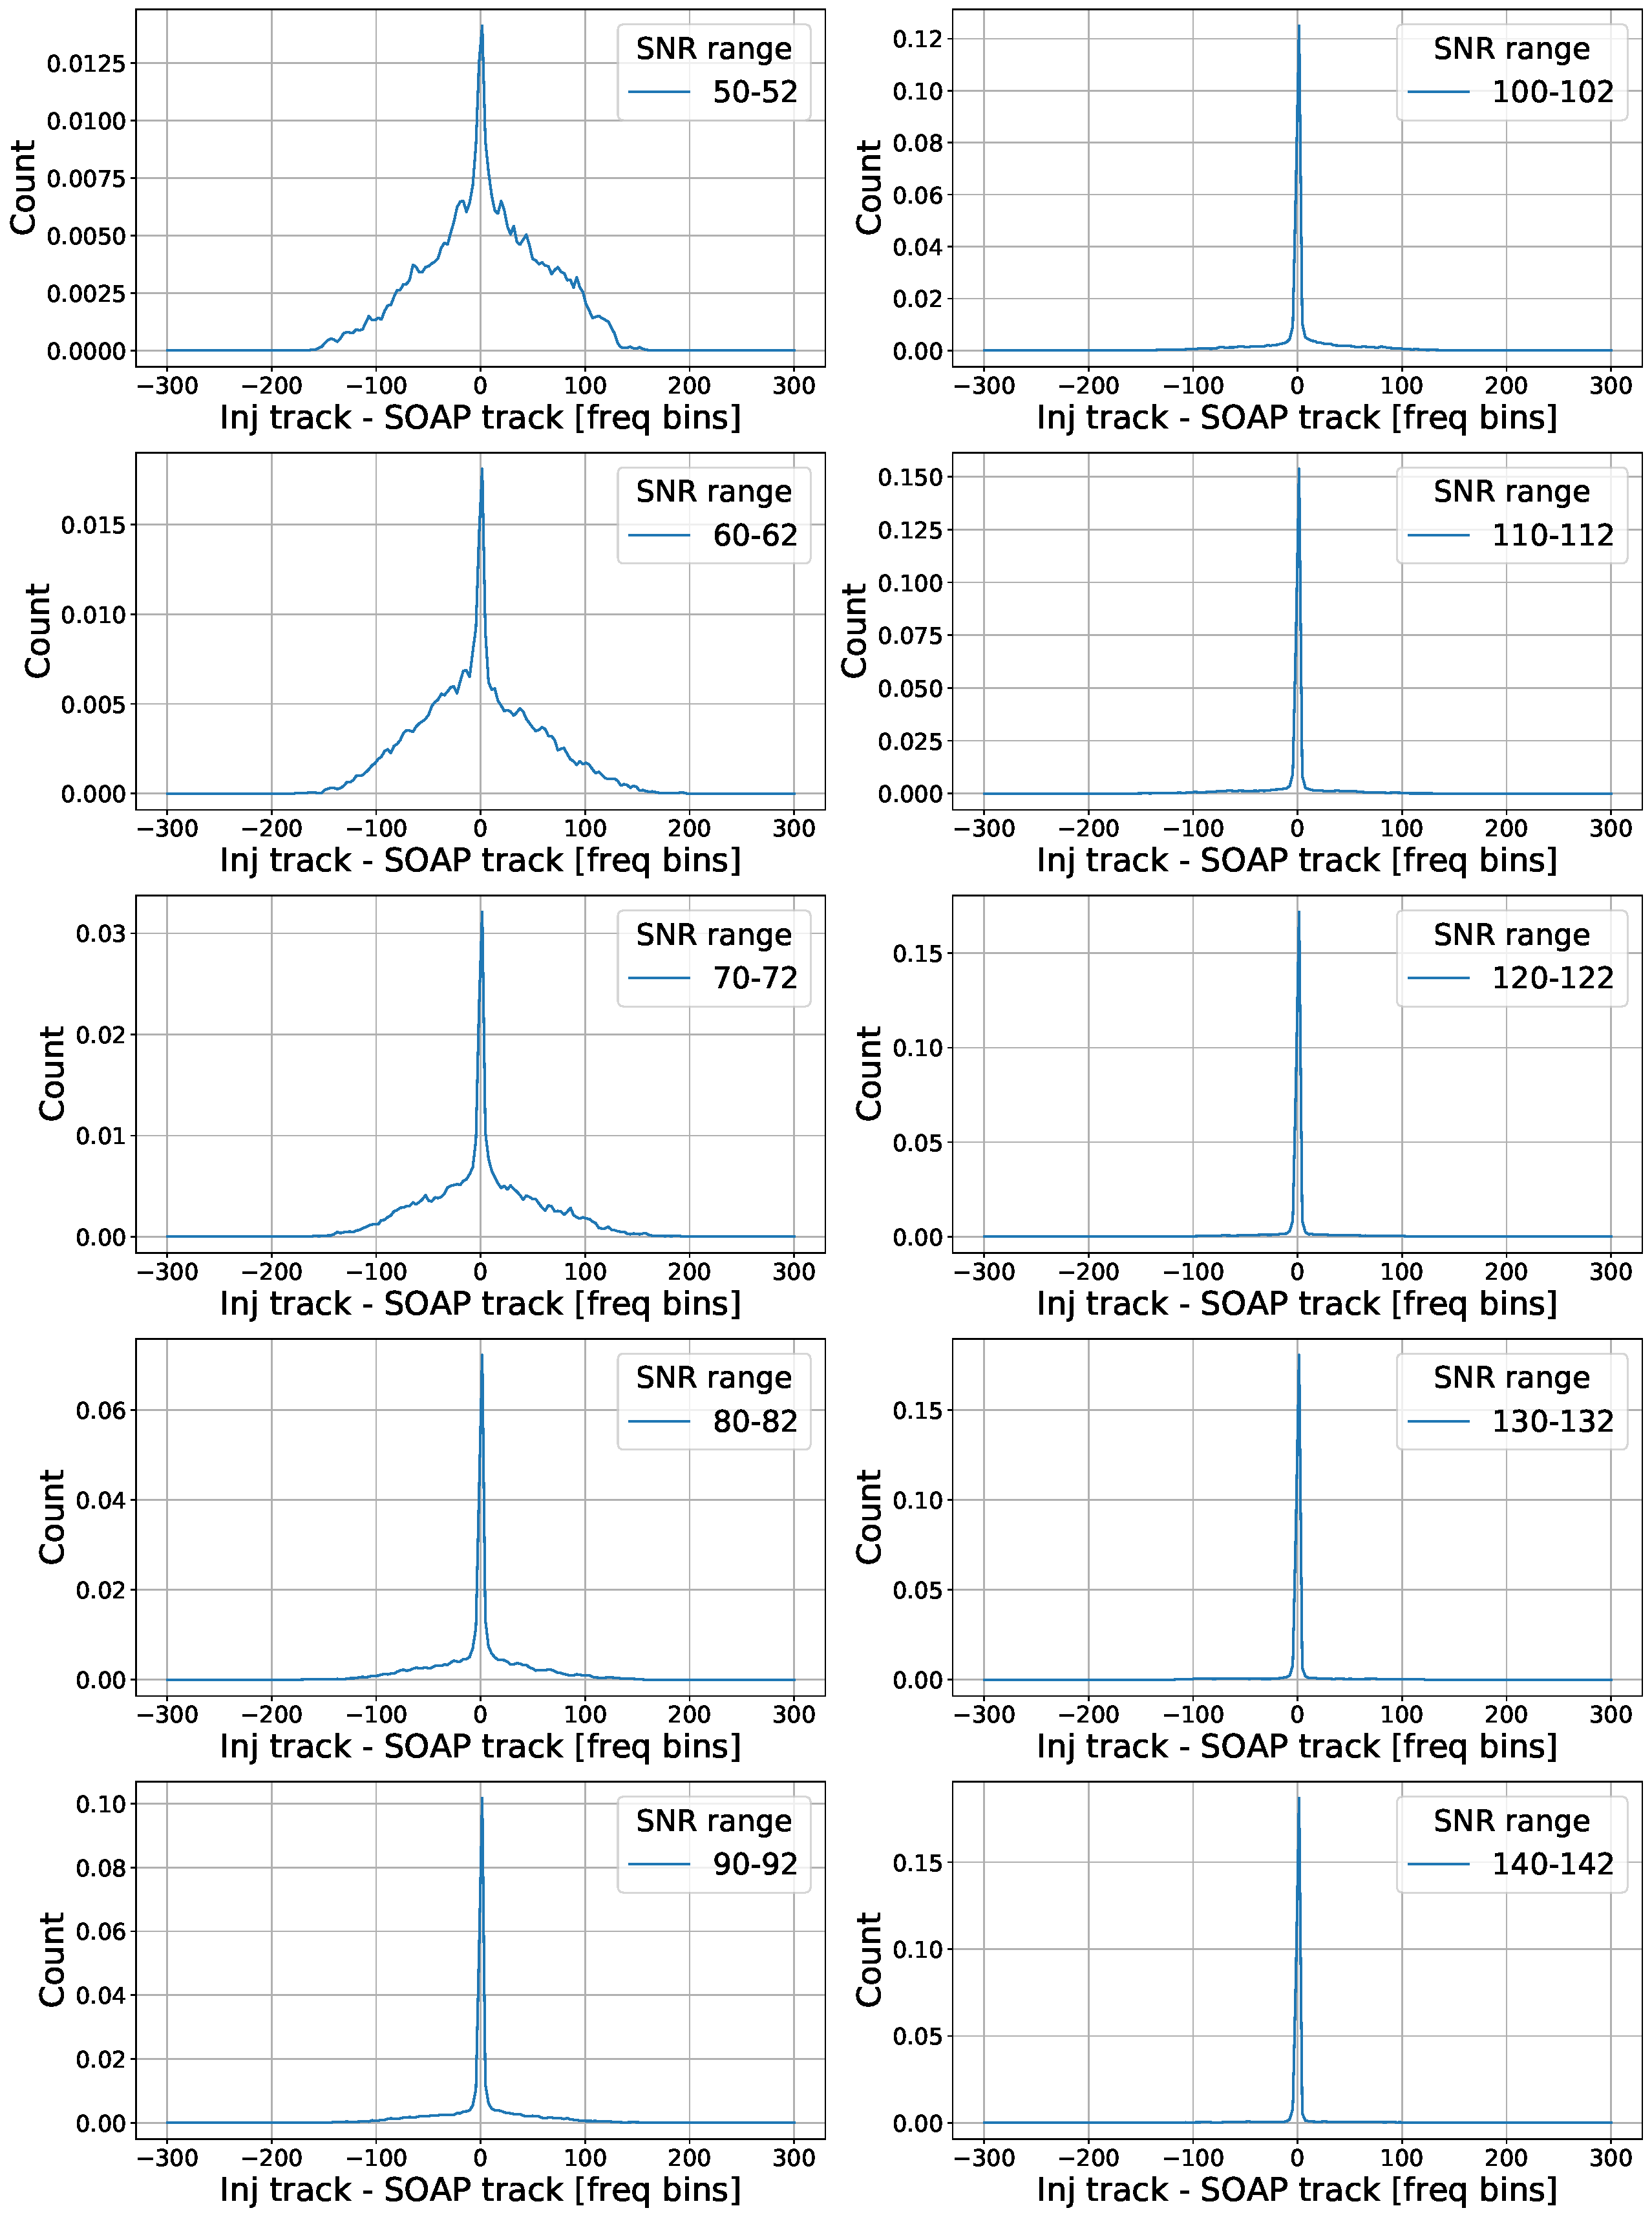
\includegraphics[width=\linewidth]{C5_parameter/KDE_range_50_100.pdf}
    \caption[KDE of likelihood in different \gls{SNR} ranges]{This figure shows
the \gls{KDE} estimates of the probability density of the differences between
the simulated (injected) \gls{CW} frequency track and the recovered Viterbi
track for a number of \gls{SNR} ranges. The difference in the tracks is
measured in discrete frequency bins. Each \gls{KDE} is generated from $\sim
300$ simulations which each have $\sim 400$ elements in their frequency tracks.
This shows a subset of the binned likelihoods between the range of \gls{SNR} 50
and 150.~\chris{stylistically you could tidy up the x-axis labels and you
should really replace "count" with the actual KDE value. If you used subplot
you could indicate the SNR bins in subcaptions.}} \label{par_est:bayes:likelihood:kde142}
    \end{figure}
%

This does introduce~\chris{shouldn't start a paragrpah like this - assuming
what you were last talking about} one more parameter to search over in our
Bayesian model, which is the \gls{SNR} $\rho$ of the signal.  The \glspl{KDE}
$\mathcal{L}$ are then used in the likelihood function $p(\bm{V} \mid
\bm{\theta}, \rho, I)$ in the Bayesian model in~\chris{3 "in"s in a row}
Eq.~\ref{par_est:bayes:eqn}, where we now have five parameters in our model
$\alpha, \delta, f, \dot{f}$ and $\rho$.  Our likelihood where we assume
independent track elements for a given Viterbi track is
%
\begin{equation} 
p(\bm{V} \mid \bm{\theta}, \rho, I) = \frac{1}{N}\prod_{i =
1}^{N} \mathcal{L}(M_i(\bm{\theta}) - V_i, \rho) , 
\end{equation} 
%
\chris{why do  you divide by $N$. I'm pretty sure that you shouldn't be doing
this} where $N$ is the length of the Viterbi track $\bm{V}$. \chris{It's not clear
exactly how the SNR is dealt with here. You haven't mentioned any binning in
which case you should index the KDE functions with an SNR dependent index.} 

% Not currently doing this 
\if
As the likelihood $\mathcal{L}$ is binned in \gls{SNR} $\rho$, and $\rho$ is a
continuous value, the likelihood is calculated as the weighted sum of the
surrounding likelihood bins, where the weights are the fractional separation of
$\rho$ from the bin centers.  
\fi

%
\subsection{Prior}
%
We set up a simple prior which does not assume much about the parameters, other
than limits on their range~\chris{too relaxed sentence - be more scientific.
Setting flat priors is NOT the same as being indifferent to the parameter
priors - it's a specific simple choice}.  We use a flat prior for $\alpha$
between $[0,2\pi]$, a flat prior in $\sin{\delta}$ between [-1,1], a flat prior
in $f$ in the range of the 0.1 Hz wide sub-band which SOAP searched through, a
flat prior in the frequency derivative in the range
$[-1e^{9},1e^{9}]$~\chris{units} and a flat prior for the \gls{SNR} $\rho$ in
the range $[50,200]$~\chris{the sky prior is obvioulsy physically motivated as
is the frequency prior over such a narrow band. It's only the SNR prior that
you would need to defend.}.


\clearpage

%%%%
%%%%
\section{\label{par_est:results}Results}
%%%%
%%%%

The method described in Sec.~\ref{par_est:bayes} takes in a Viterbi track and uses this to estimate the five dimensional posterior distribution $p\left(\left\{ \alpha, \delta, f, \dot{f}, \rho \right\} \mid \bm{V}, I \right)$.
To calculate this posterior we use a technique known as nested sampling, specifically the package {\it Dynesty} \citep{speagle2019DynestyDynamic}, which is explained in Sec.~\ref{intro:prob:bayes}. \joe{will explain more in the return of intro chapter}

As an example of what this returns, we can first simulate a \gls{CW} signal with parameters 
\begin{equation}
    \label{par_est:results:examplepars}
    \begin{split}
        \alpha &= 4.2 \; \rm{rad}\\
        \delta &= -0.06 \; \rm{rad} \\
        f &= 148.23 \; \rm{Hz}\\
        \dot{f} &= -3.55e-15 \; \rm{Hz/s}\\
        \rho &= 151,\\
    \end{split}
\end{equation}

and generate the associated spectrograms for the \gls{LIGO} detectors H1 and L1.
The SOAP search from chapter \ref{soap} is then run using the line-aware statistics the same parameters as in Tab.~\ref{soap:results:parameters}, the output Viterbi track is then plotted with the \gls{CW} frequency track in Fig.~\ref{par_est:results:freqtrack}. 
%
\begin{figure}[ht]

    \centering
    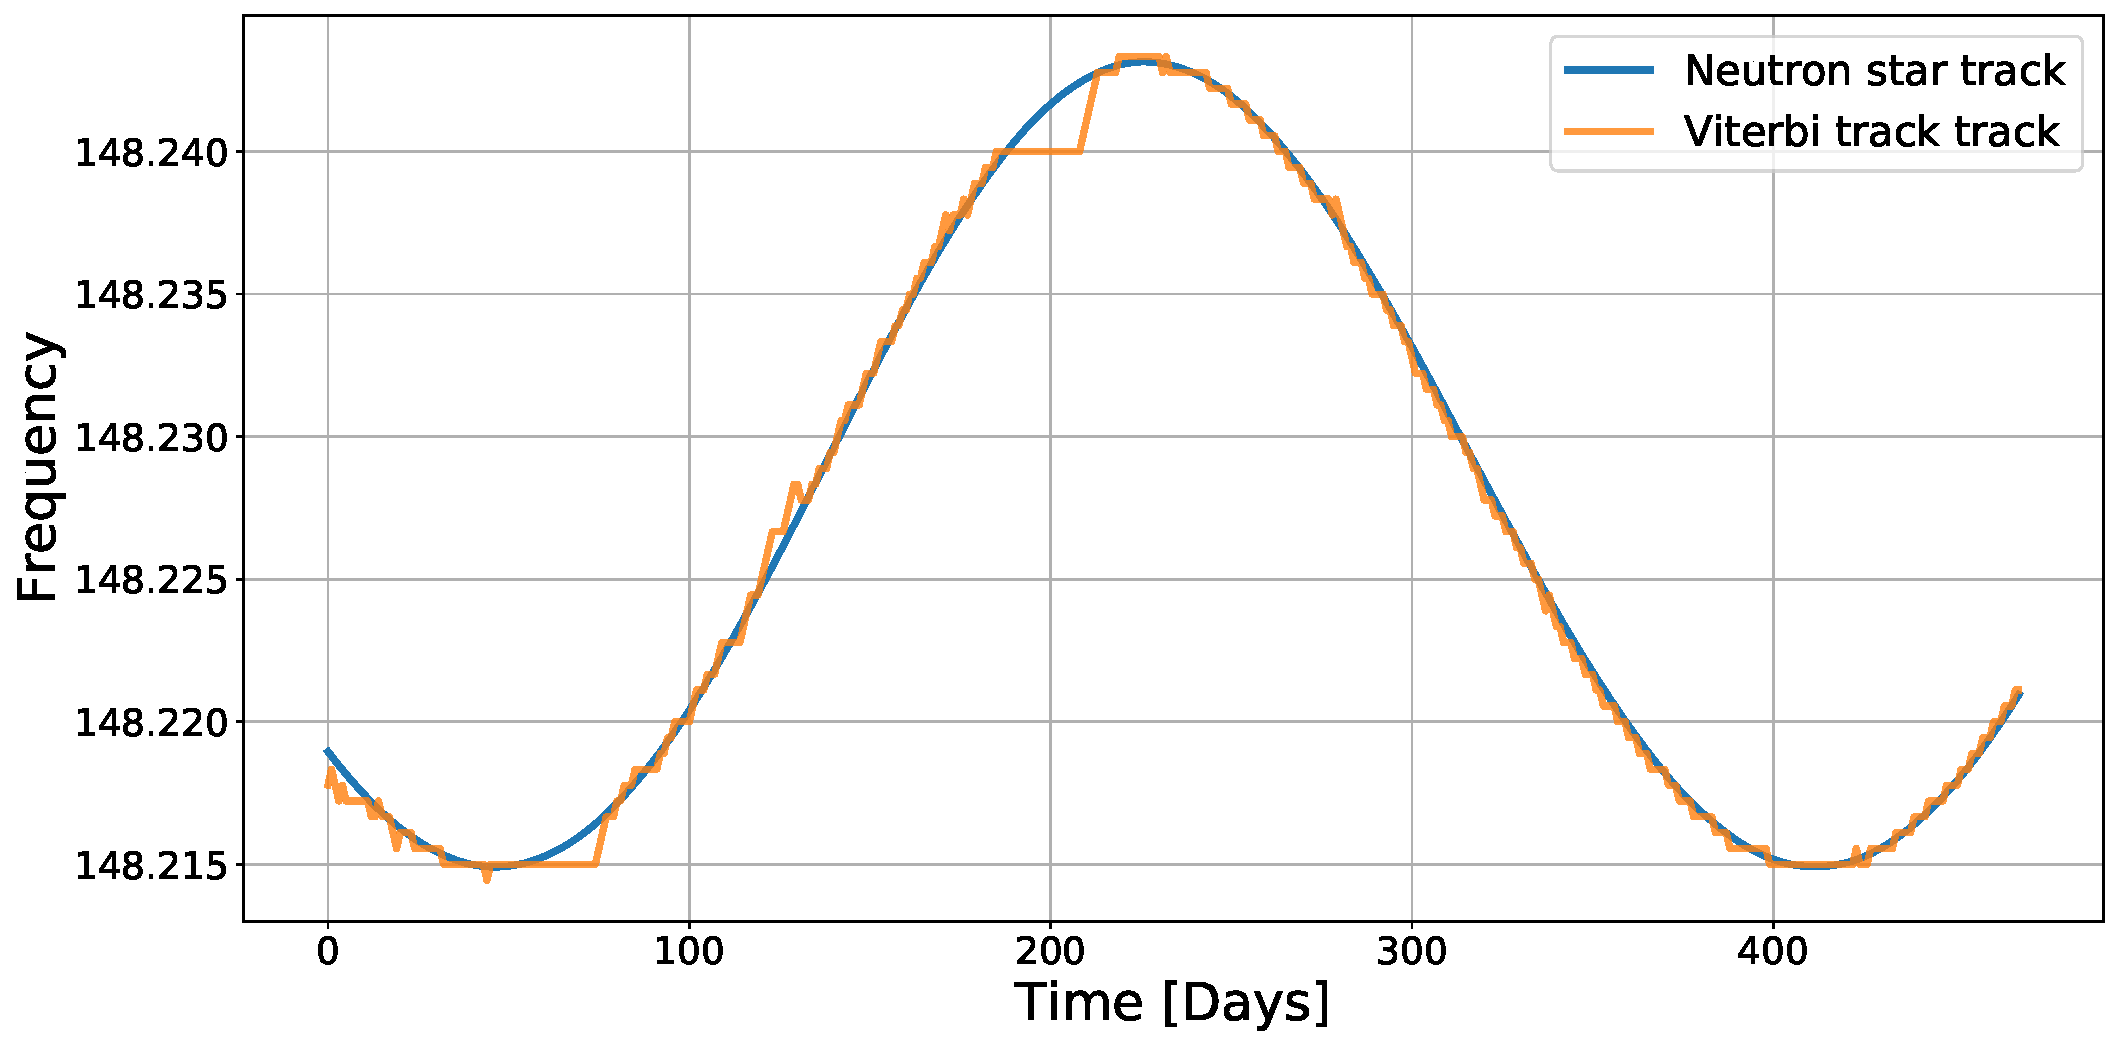
\includegraphics[width=\linewidth]{C5_parameter/example_freqtrack.pdf}
    \caption[Frequency track of injected signal]{ Example simulated \gls{CW} frequency using parameters in Eq.~\ref{par_est:results:examplepars} and the Viterbi track recovered from the simulation. The track is samples once per day, where the oscillation visible here is due to the Doppler modulation of the Earth's orbit.}
    \label{par_est:results:freqtrack}
    
\end{figure}
%
In this case the Viterbi track can be seen to closely follow the simulated \gls{CW} frequency track.

The Bayesian analysis described in Sec.~\ref{par_est:bayes} is then run using this Viterbi track as input, where this returns the posterior distribution shown in Fig.~\ref{par_est:results:example_posterior}.
In this example, the injected parameter values (marked in orange) are contained within the marginal posterior distributions for all of the parameters excluding the \gls{SNR}.
The distribution in \gls{SNR} appears to have hard edges at the edge of the binned likelihood function, which begins to demonstrate some problems with the definition of the likelihood, however,I will describe this more in Sec.~\ref{par_est:results:simulations}.
%
\begin{figure}[pt]

    \centering
    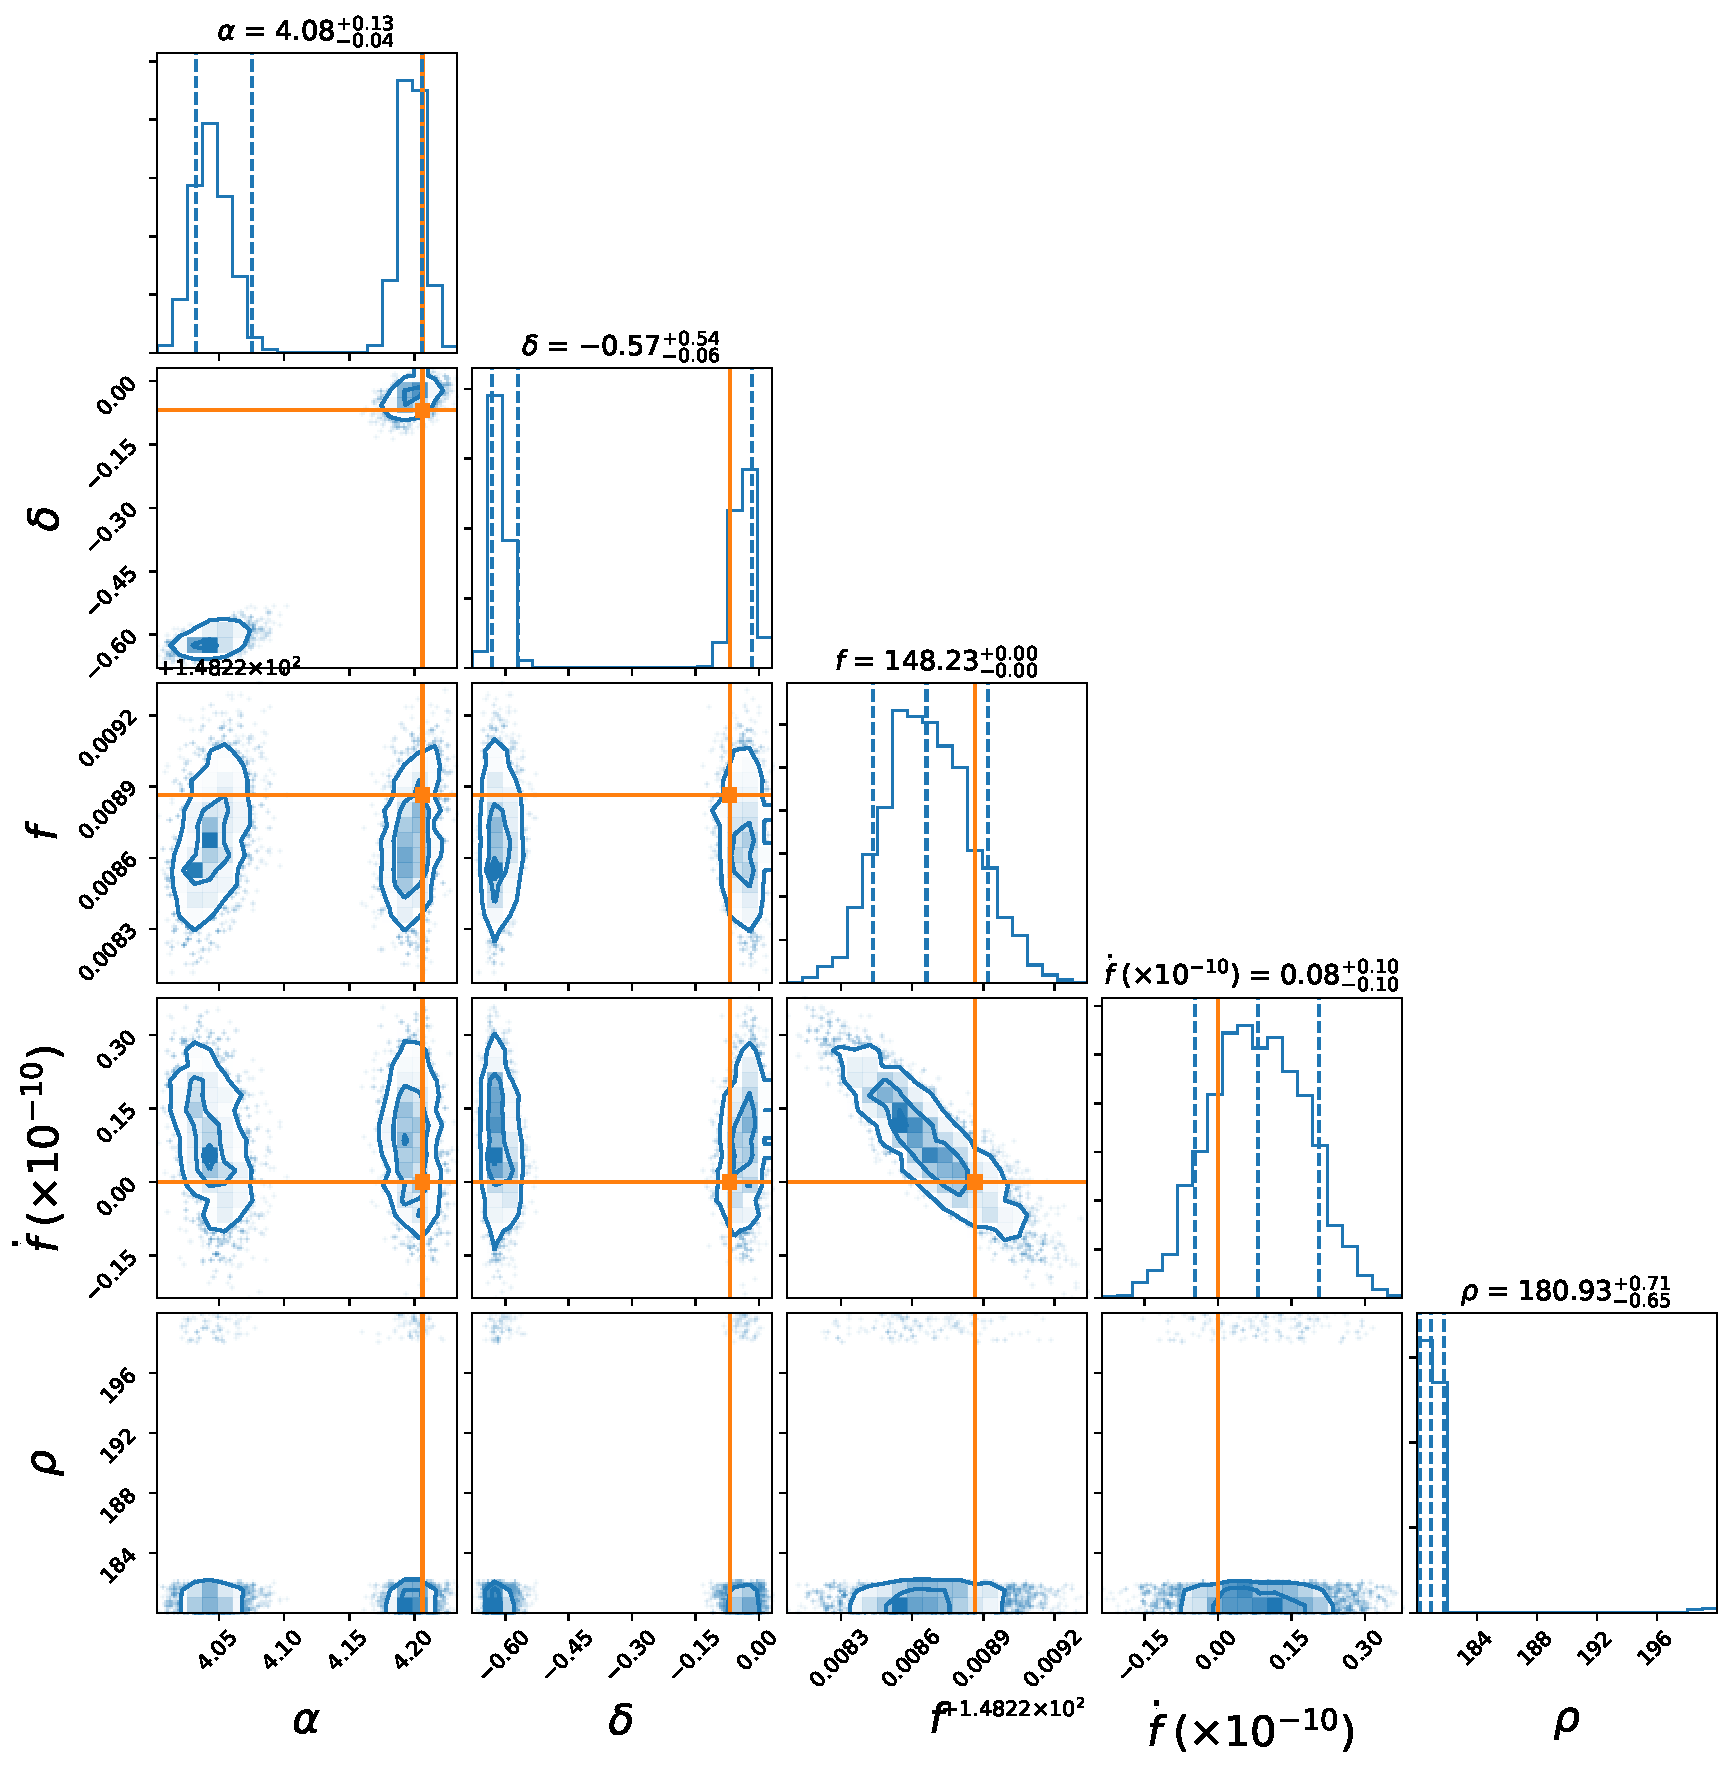
\includegraphics[width=\linewidth]{C5_parameter/cornerplot.pdf}
    \caption[KDE of likelihood in different \gls{SNR} ranges]{This figure shows an example of the posterior distribution of a signal with \gls{SNR} 151. Each panel shows the marginal distributions for each parameter, where the parameters used for the simulation are marked in orange. In this example each of the posteriors match well with the injected parameters, but the sky position is bimodal. }
    \label{par_est:results:example_posterior}
    
\end{figure}
%

The marginal posterior distribution of the sky parameters is easier to interpret it is projected onto a sky map, therefore, Fig.~\ref{par_est:results:example_skypos} the parameters $\alpha$ and $\delta$ are shown on a sky projection in the ecliptic frame.
The sky position parameters $\alpha,delta$ of the \gls{CW} signal are in the equatorial coordinate system, therefore these have been transformed into the ecliptic frame $\beta,\gamma$ such that the sky position posteriors easier to interpret.
The Viterbi tracks and \gls{CW} frequency tracks used in this analysis are sampled once a day, therefore, we should only see the doppler modulation from the orbit of the earth around the sun.
In the ecliptic frame, i.e. where the $z$ axis is perpendicular to the orbital plane of the earth, for any ecliptic longitude, there are two sky positions at opposite ecliptic latitudes which will return the same frequency track. 
This then means that we would expect the marginal posterior distribution to have two modes on the sky at these two locations, where this is seen in \ref{par_est:results:example_skypos}.

%
\begin{figure}[ht]
    \centering
    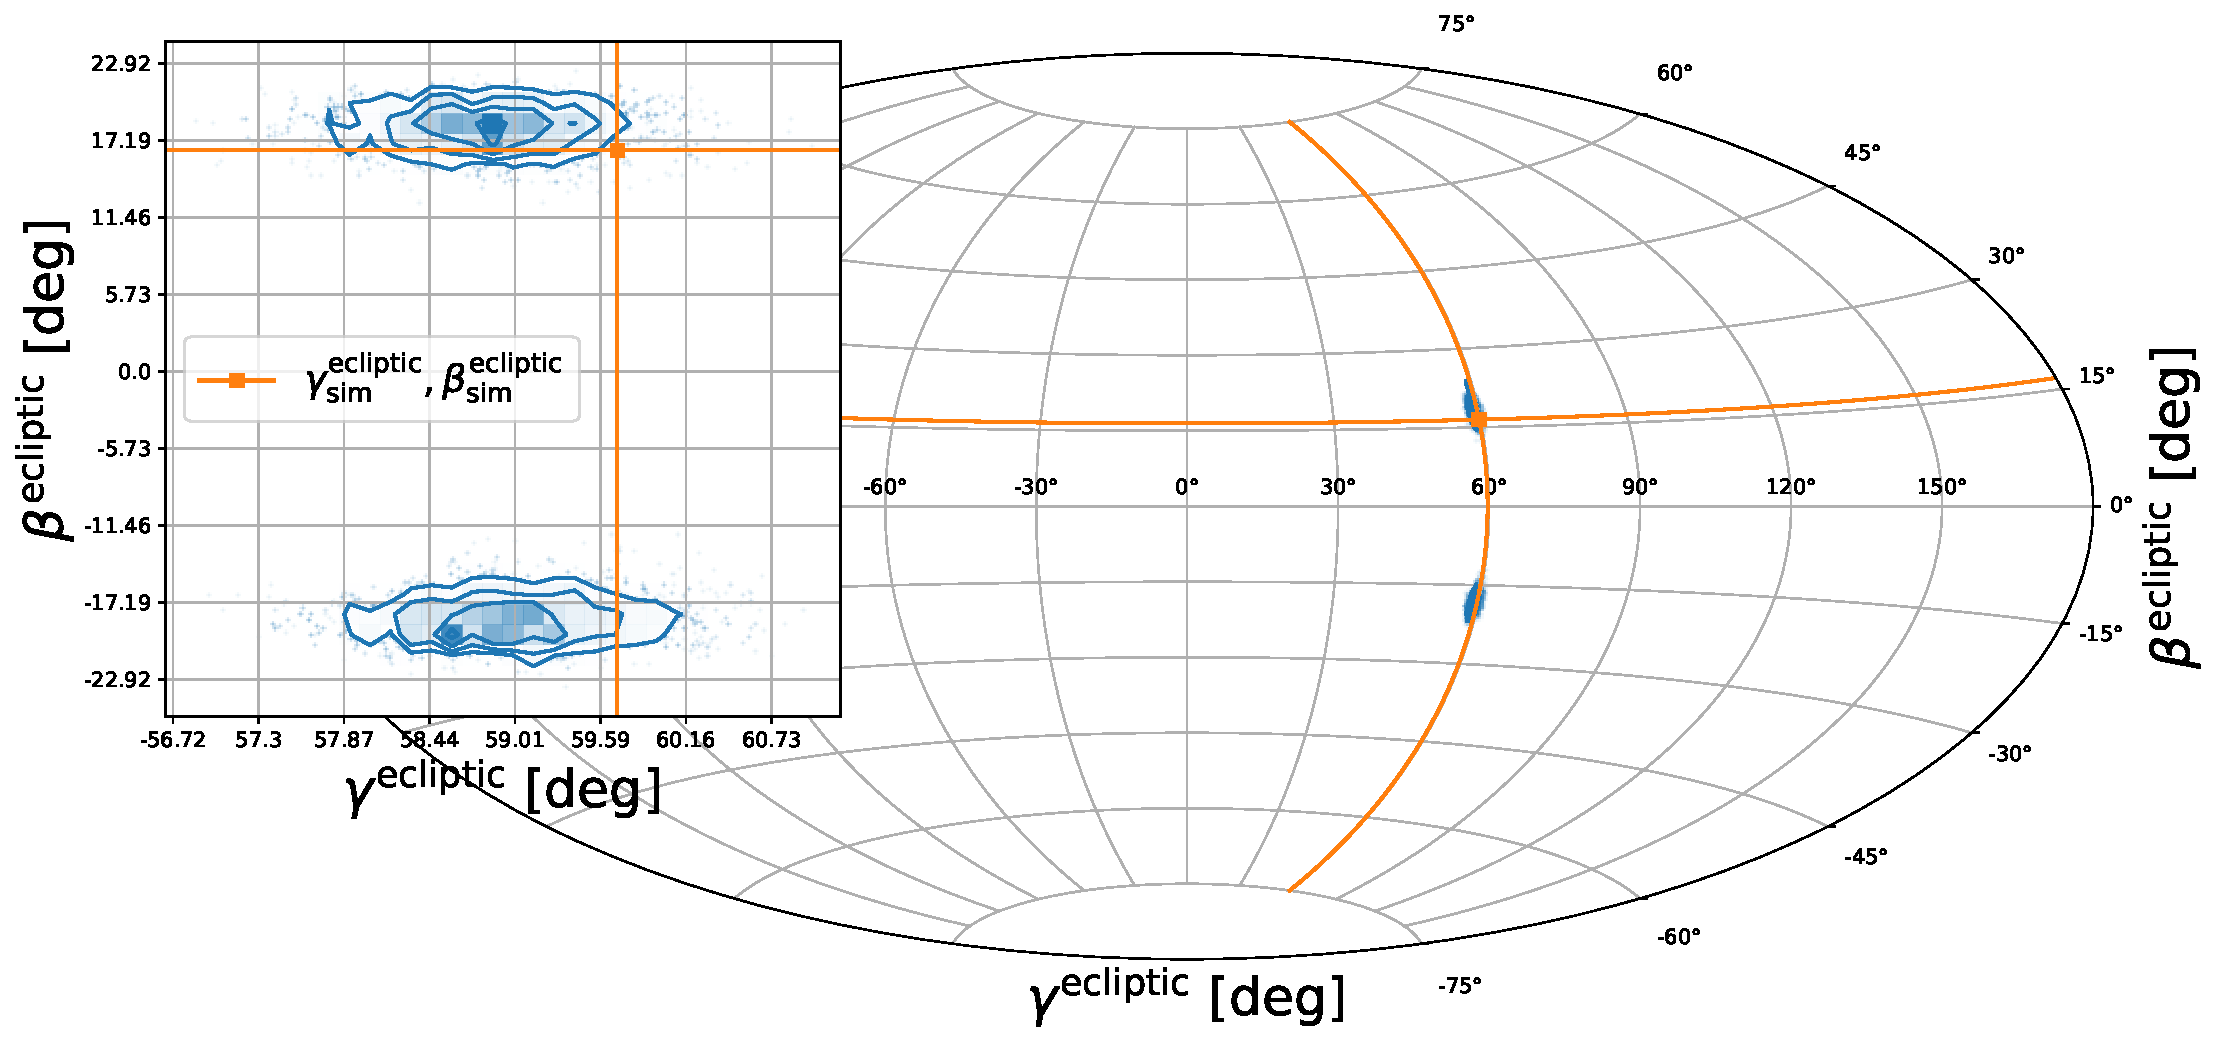
\includegraphics[width=\linewidth]{C5_parameter/skypos_ecliptic.pdf}
    \caption[Example of posterior of sky position in ecliptic frame]{This figure shows an example of the marginal posterior distribution of the sky position in the ecliptic frame $\alpha^{\rm{ecliptic}},\delta^{\rm{ecliptic}}$ of a signal with \gls{SNR} 144. The overlaid panel is a zoomed area around the posterior distribution, where the orange marker shows the injected parameters.}
    \label{par_est:results:example_skypos}
    
\end{figure}
%

%
%
\subsection{\label{par_est:results:simulations}Simulations}
%
%
To test this method, we generate a set of simulations in Gaussian noise, where we generate spectrograms of \gls{CW} signals as in Sec.~\ref{soap:results} and Sec.~\ref{machine:results}.
This is the same simulated test set from Sec.~\ref{machine:results}, where \gls{CW} signals were injected into 50\% of the 0.1 Hz wide sub-bands between between 40 and 500 Hz, with the parameters as described in Tab.~\ref{machine:data:injections:table}. 
The SOAP search using the line aware statistic with parameters in Tab.~\ref{soap:results:parameters} is run on each sub-band, where the Viterbi track and \gls{CW} signal parameters $\alpha, \delta, f, \dot{f}$ associated with each simulation are recorded.
The Viterbi track can then be used to run the Bayesian analysis described in Sec.~\ref{par_est:bayes}.
In these simulations, we have 2300 simulated signals which have an \gls{SNR} range between 20 and 200, where for this test we randomly select 200 of these simulations.

\if
However, as the \gls{SNR} of the simulations decreases, the probability of SOAP identifying the signal decreases, therefore, we only want to run the Bayesian parameter estimation on signals which are most likely to be astrophysical.
Therefore, as in Sec.~\ref{soap:results}, we find the false alarm rate, which is the fraction of bands which contain no injection and has a Viterbi statistic which exceeds a given threshold, where this is set to 0\% for this test.
We can then select all of the sub-bands which have a Viterbi statistic above this threshold for further investigation, where with a 0\% false alarm rate we have 2000 \joe{ecaxt number} injections to investigate.
The Viterbi statistics for each of these injections can be seen in Fig.~\ref{par_est:results:all_viterbi}, where the 0\% false alarm value is marked.
%
\begin{figure}
    \centering
    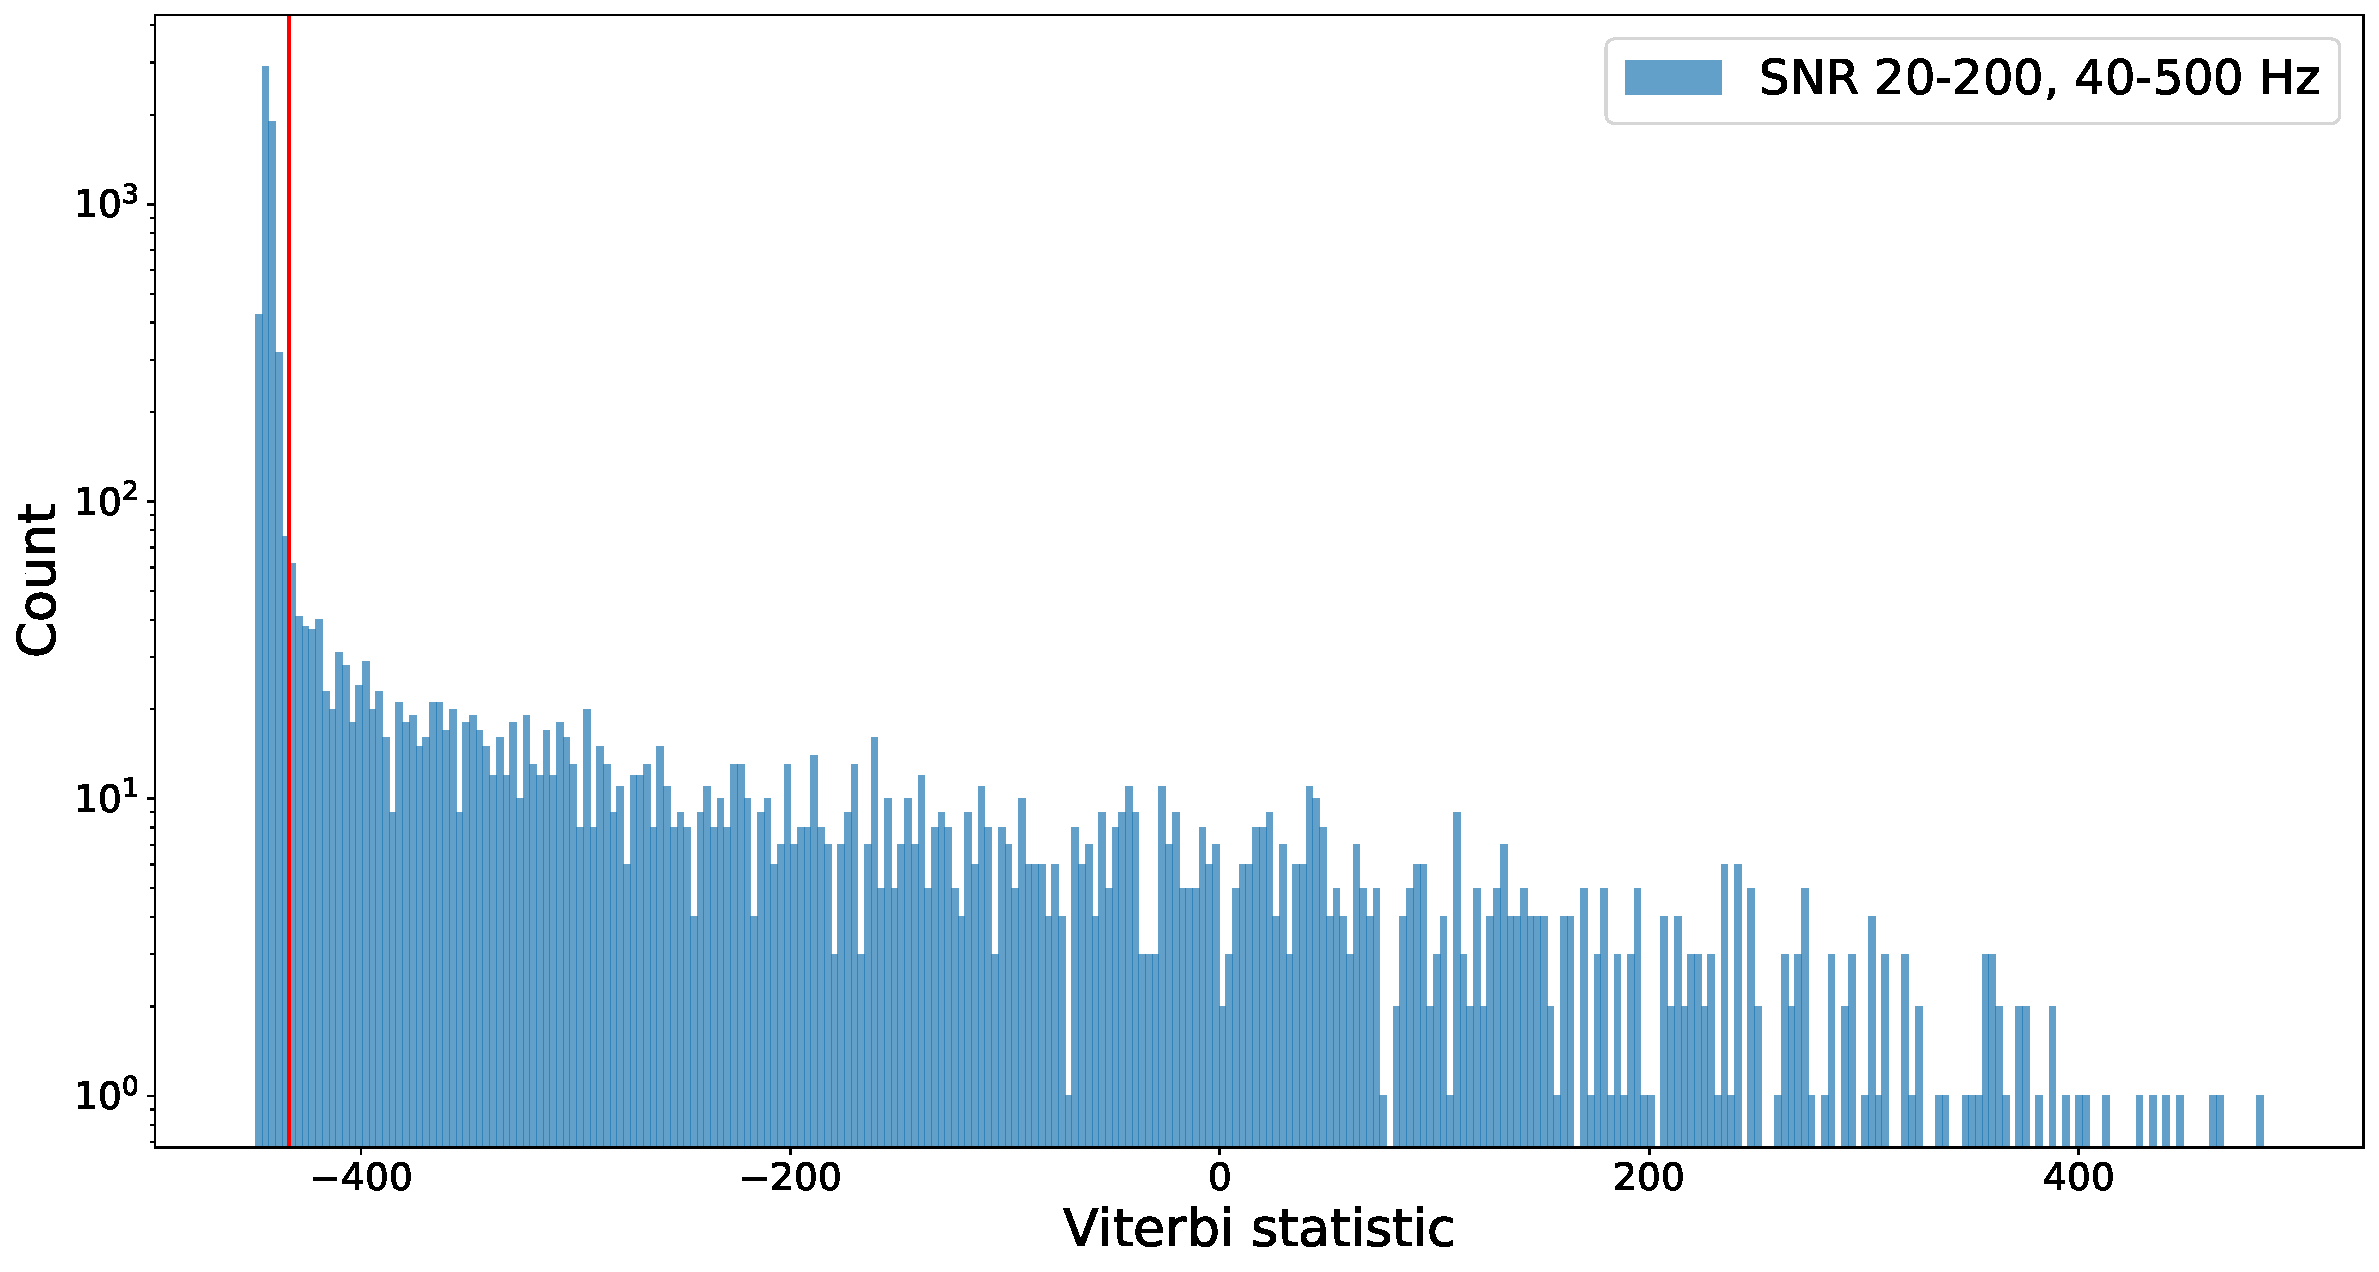
\includegraphics[width=\linewidth]{C5_parameter/viterbi_hist.pdf}
    \caption[All Viterbi statistics]{This figure shows a histogram of the Viterbi statistics from each of the 0.1 Hz wide sub bands in this test. \joe{more}}
    \label{par_est:results:all_viterbi}
\end{figure}
\fi


\subsubsection{\label{par_est:results:simulations:ppplot}P-P plot}

The p-p plot is a mechanism to validate the effectiveness of the Bayesian model and computation using many simulations.
From Sec.~\ref{par_est:results} we have the output posterior distribution $p(\bm{\theta} \mid \bm{V}, I)$, or more correctly we have $N$ samples from this distribution $\bm{\theta}_i$, and we have the injected parameters $\bm{\theta}_{\rm{inj}}$.
For each simulation, we can calculate the posterior quantile $q(\theta_{\rm{inj}})$ from the marginal posterior distribution
\begin{equation}
    q(\theta_{\rm{inj}}) = P(\theta_{\rm{inj}} > \theta) = \frac{1}{N} \sum_{i=1}^{N} H(\theta_{\rm{inj}} - \theta_i),
\end{equation}
where $H(x)$ is the Heaviside step function. 
This calculates the fraction of the marginal posterior distribution which has a parameter $\theta$ less than the injected parameter $\theta_{\rm{inj}}$ \citep{cook2006ValidationSoftware}.
If the Bayesian model and computation of the posterior is valid, then as the number of samples approaches infinity ($N \rightarrow \infty$), the posterior quantile $q(\theta_{\rm{inj}})$ should follow a uniform distribution $[0,1]$ \citep{cook2006ValidationSoftware}.
This then provides a method to check the validity of our analysis.

For each of our simulations we can calculate $q(\theta_{\rm{inj}})$, such that we have values $\bm{q}_{\theta}$, where the fraction of simulations which fall within a given \gls{CI} $C$ is the cumulative distribution of $\bm{q}_{\theta}$, i.e. $P(\bm{q}_{\theta} > C)$, where $C$ ranges between $[0,1]$.
If $q(\theta_{\rm{inj}})$ and therefore $\bm{q}_{\theta}$ follows a normal distribution, then $P(\bm{q}_{\theta} > C) = C$ \citep{cook2006ValidationSoftware}.
Plotting $P(\bm{q}_{\theta} > C)$ against $C$ for each parameter $\theta$, then shows the fraction of simulations which have a $q(\theta_{\rm{inj}})$ within some \gls{CI} $C$, this is known as a p-p plot.

If the analysis is valid, i.e the marginal posterior distributions agree with the injected parameters, then this plot should follow a straight diagonal line, indicated by the black line in Fig.~\ref{par_est:results:ppplot_example}.
If the marginal posterior distribution is shifted to right of the injected parameters, shown in the first panel of Fig.~\ref{par_est:results:ppplot_example}, i.e. the true value lies in the lower tail of the posterior for each simulation, then the p-p plot will show a curve above the diagonal.
Similarly, if the marginal posterior distribution is shifted to left of the injected parameters, shown in the second panel of Fig.~\ref{par_est:results:ppplot_example}, i.e. the true value lies in the upper tail of the posterior for each simulation, then the p-p plot will show a curve below the diagonal. 
If the posterior is under constrained shown in the third panel of Fig.~\ref{par_est:results:ppplot_example}, i.e. the posterior is wider than the perfectly recovered posterior, then the curve will follow an S shape where the S is below the diagonal at $C < 0$.5 and above the diagonal at $C > 0.5$.
Similarly, if the posterior is over constrained shown in the fourth panel of Fig.~\ref{par_est:results:ppplot_example},i.e. the posterior is narrower than the perfectly recovered posterior, then the curve will follow an S shape where the S is above the diagonal at $C < 0.5$ and below the diagonal at $C> 0.5$.
%
\begin{figure}[ht]
    \centering
    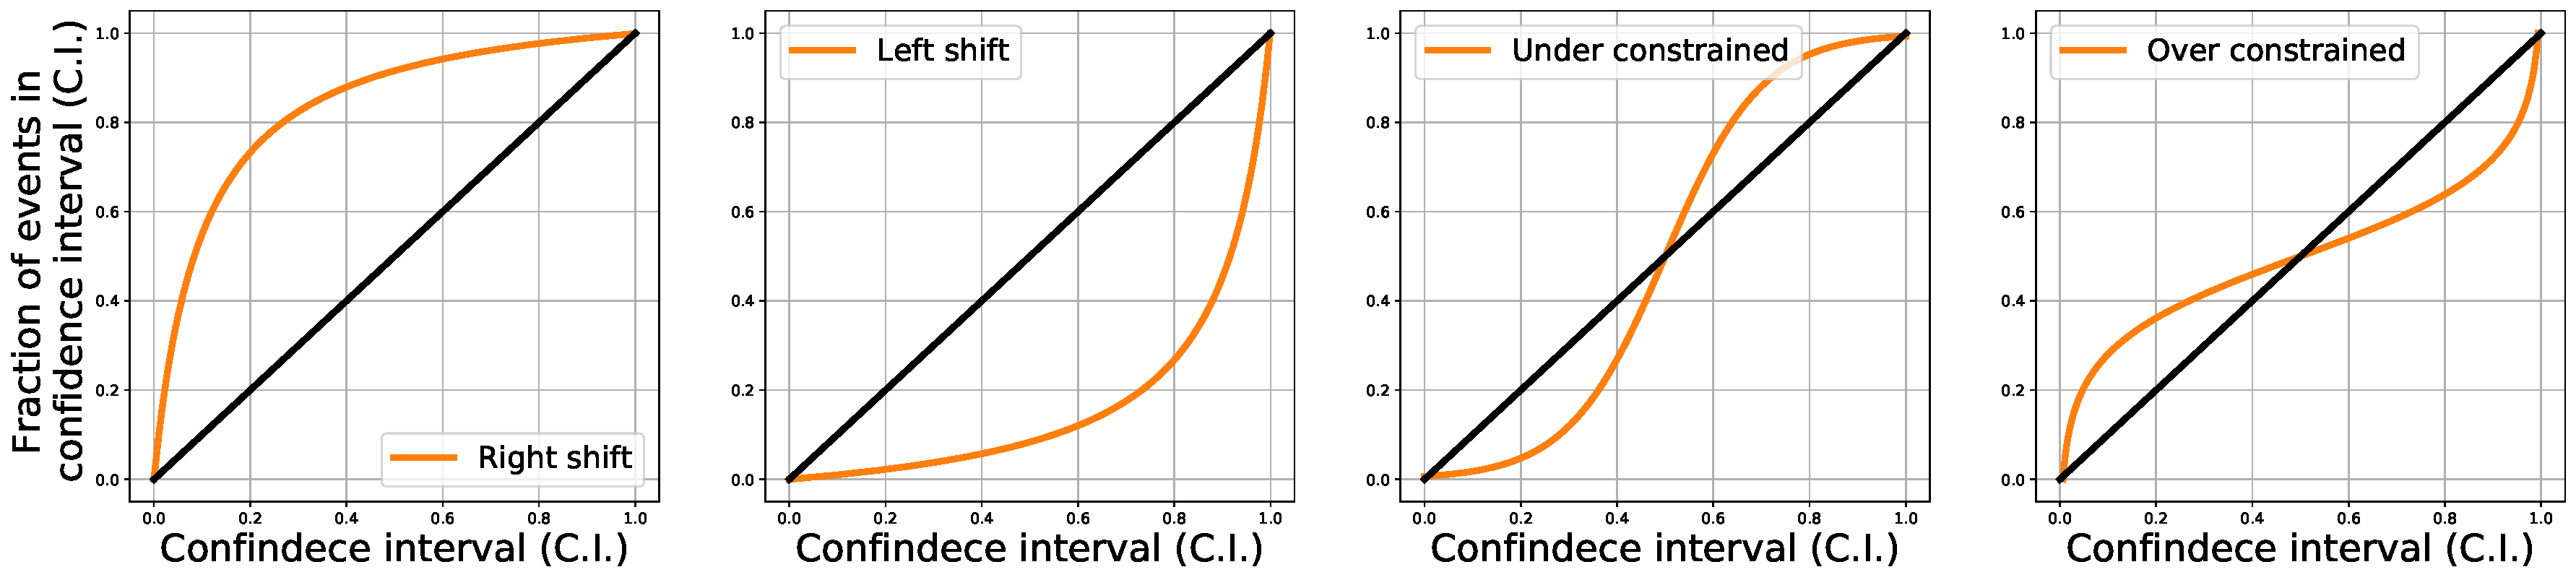
\includegraphics[width=\linewidth]{C5_parameter/ppplot_examples.pdf}
    \caption[p-p plot examples]{This figure shows examples of p-p plots for posterior distributions which are shifted to the right (larger values of the parameter), to the left (smaller values of the parameter) and over and under constrained posteriors. The black curve shows the p-p plot when the posterior distribution is perfectly recovered, i.e. the confidence intervals follow a uniform distribution.}
    \label{par_est:results:ppplot_example}
\end{figure}

Using this information, we can look at the p-p plot for the 200 simulations in this test, which is shown in Fig.~\ref{par_est:results:ppplot}.
We can see that for the parameters $f$ and $\dot{f}$ we recover an over constrained posterior distribution.
For the \gls{SNR} parameter $\rho$, the recovered posterior is both shifted to the right and is over constrained, i.e. we assume higher \glspl{SNR} than perfectly recovered distribution.
For both the right ascension parameter $\alpha$ and the declination parameter $\delta$, we can see that we recover under constrained posterior distribution.
However, as the modes are widely separated, if the true parameter lies between the two modes then it would return a \gls{CI} of $\sim 0.5$, for many simulations this would produce a p-p plot which appears as an under constrained posterior when it is actually two widely separated over constrained posteriors.
This becomes more clear when investigating the area contained within a contours of the posterior which is explained in Sec.~\ref{par_est:results:simulations:skyarea}.
%
\begin{figure}[ht]
    \centering
    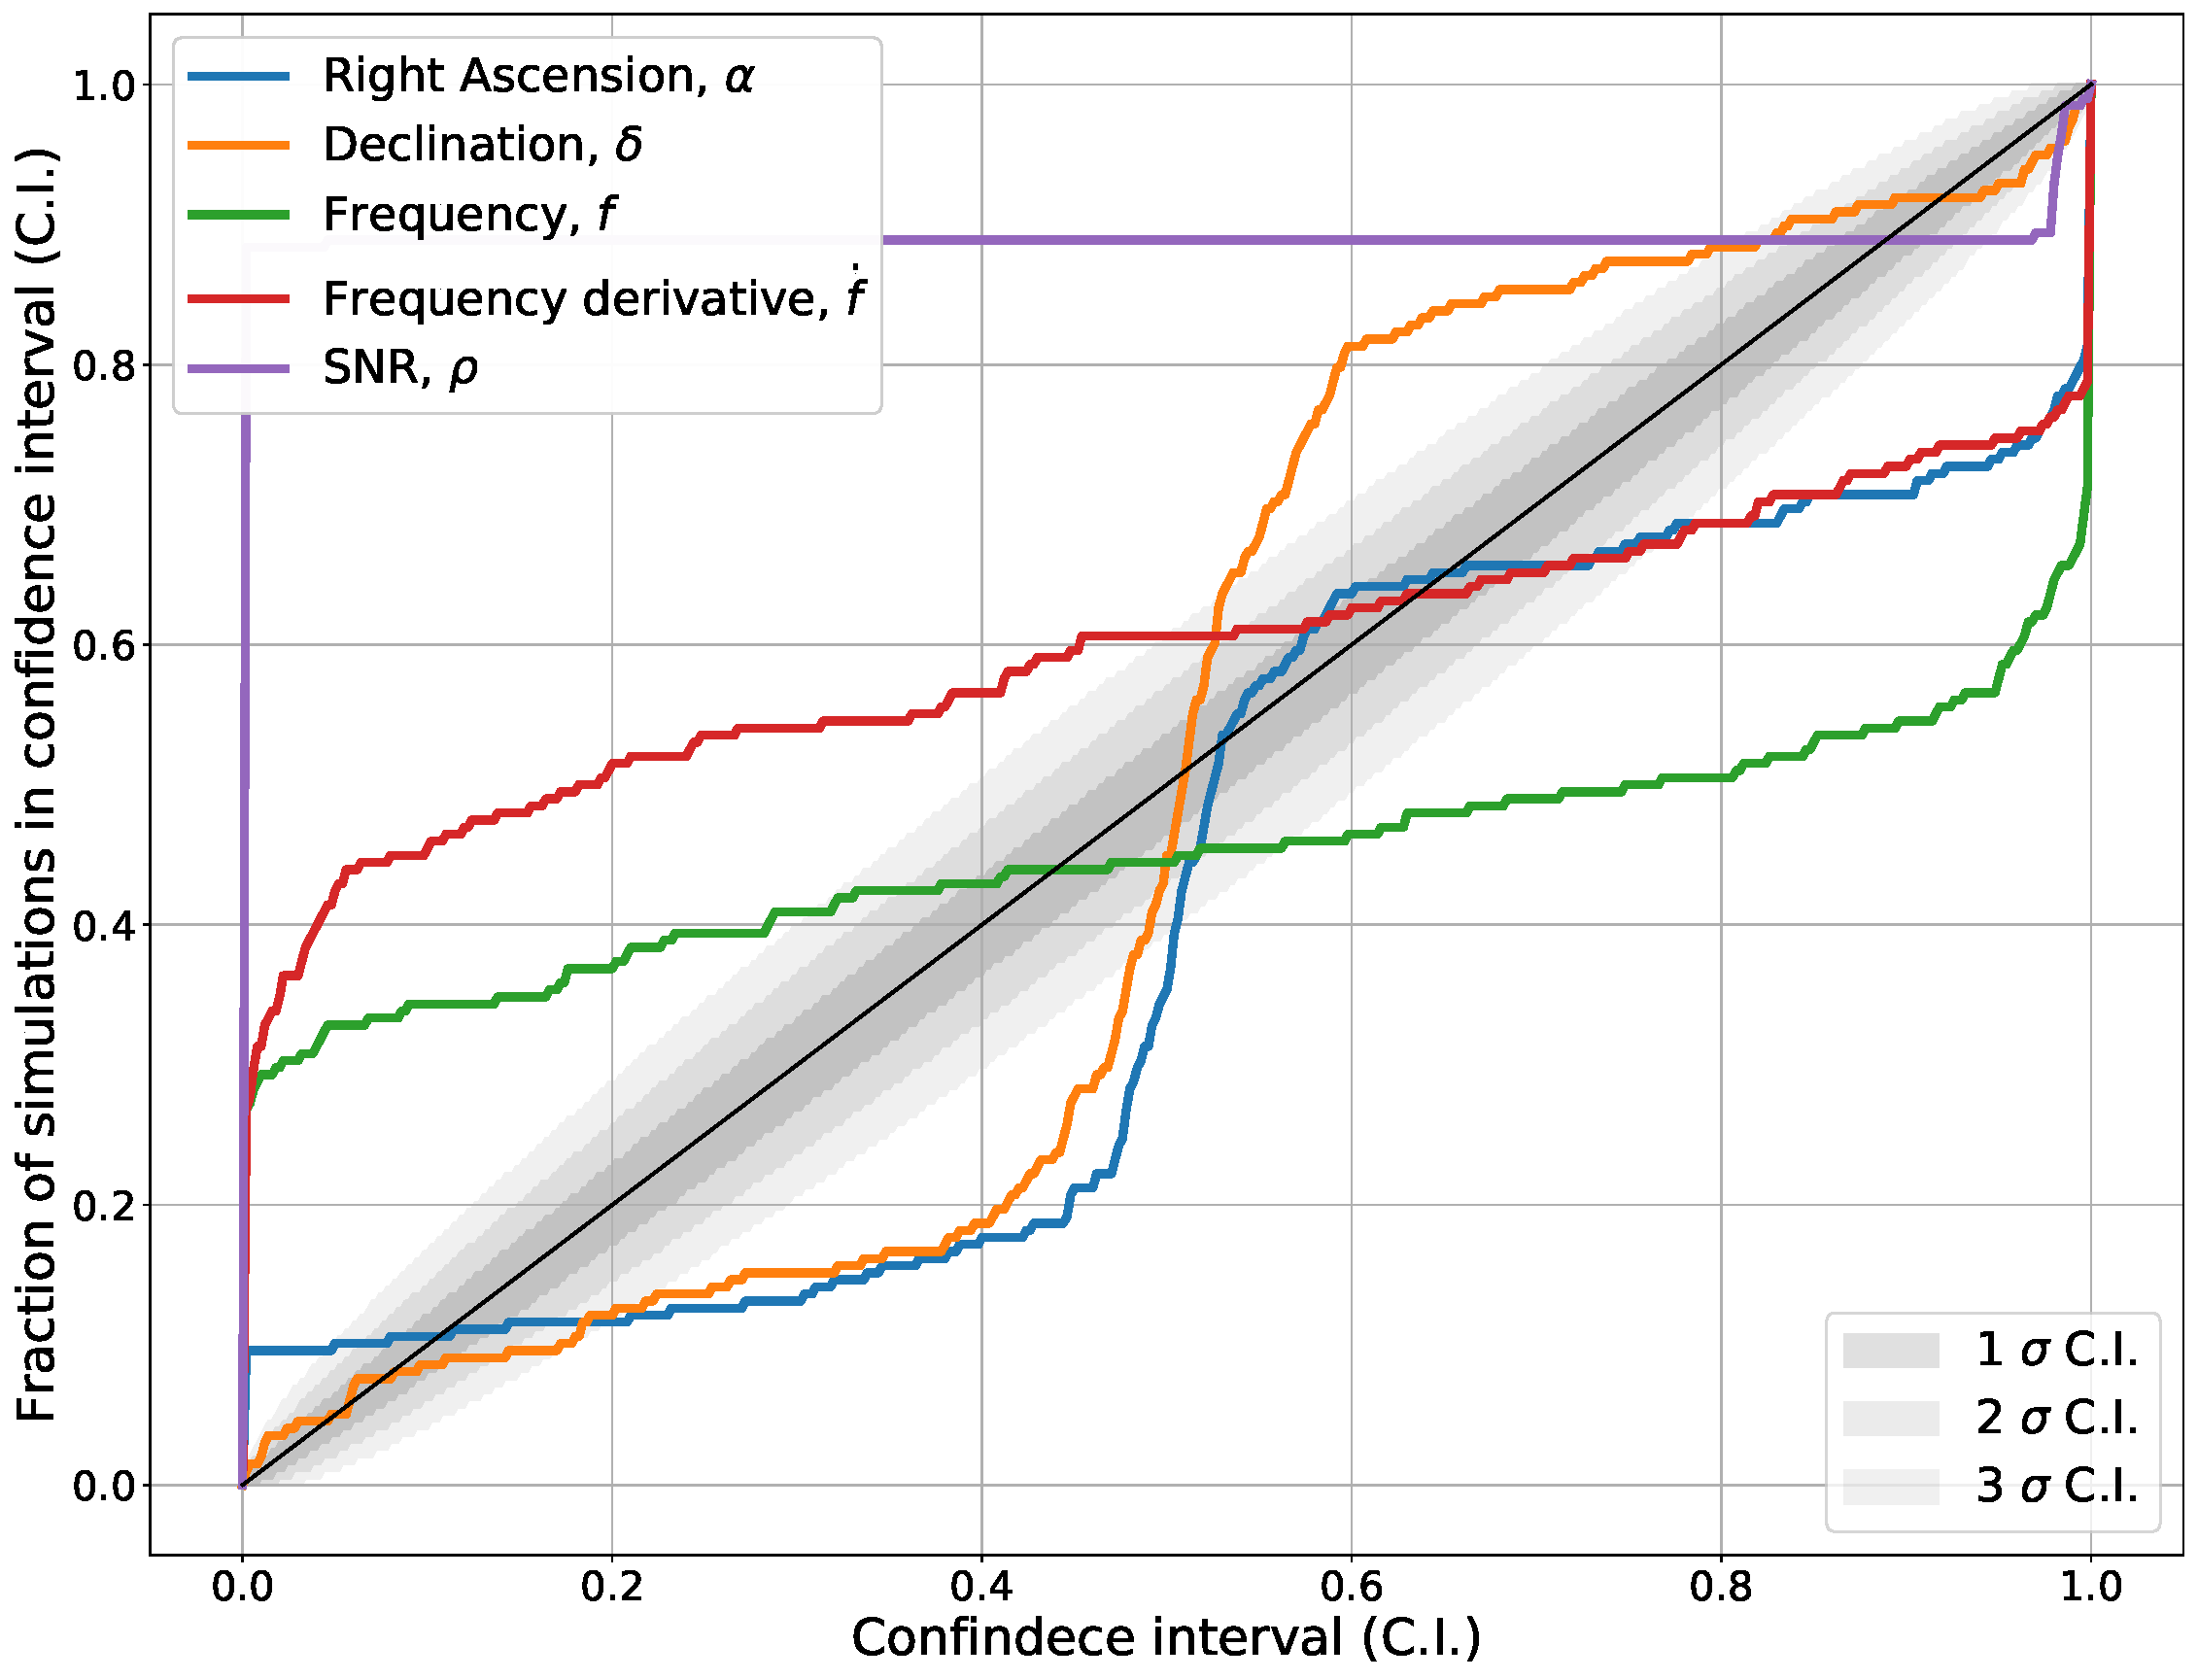
\includegraphics[width=\linewidth]{C5_parameter/ppplot.pdf}
    \caption[p-p plot for the CW simulations]{The p-p plot is shown for the 200 signals described in Sec.~\ref{par_est:results}, which range between 40 and 200 in \gls{SNR}. This describes how well the marginal posterior distributions for each parameter match the simulated parameter. The \gls{SNR}, frequency and frequency derivative are all over constrained distribution, i.e. narrower than the true distribution, and the sky position parameters $\alpha,\delta$ are under constrained.}
    \label{par_est:results:ppplot}
\end{figure}

Each of the curves in Fig.~\ref{par_est:results:ppplot} indicate that the current analysis does not correctly reproduce the true posterior distribution. 
One likely reason for this could be our definition of the likelihood in Sec.~\ref{par_est:bayes:likelihood}, here to simplify the problem we assume that all track components are independent, this is not necessarily true and could contribute to the over constrained posterior distributions. 

%
%
\subsubsection{\label{par_est:results:simulations:skyarea}Sky area at given confidence interval}
%
%

If we assume that the estimated posterior distribution is correctly recovered, i.e. it is not under constrained or shifted, then we can estimate the area of the sky which this method can localise the source to. 
To do this we can use our estimation of the marginal posterior distribution on the sky, and draw a contour on the posterior which contains 95\% of the probability.
The area contained within this contour is then the sky area which the source can be localised to at a 95\% confidence, this can be seen as the green contour in Fig.~\ref{par_est:results:sky_area_example}.
Similarly, a contour can be drawn at the values of the injected sky position parameters where the area within this contour can be found, this is shown as the red contour in Fig.~\ref{par_est:results:sky_area_example}.
If the contour at the injected parameter is much larger than the contour at 95\% confidence, then this implies that the posterior distribution is over constrained.
These two areas are another measure of the validity and ability of this method to extract the parameters. 
%
\begin{figure}[ht]
    \centering
    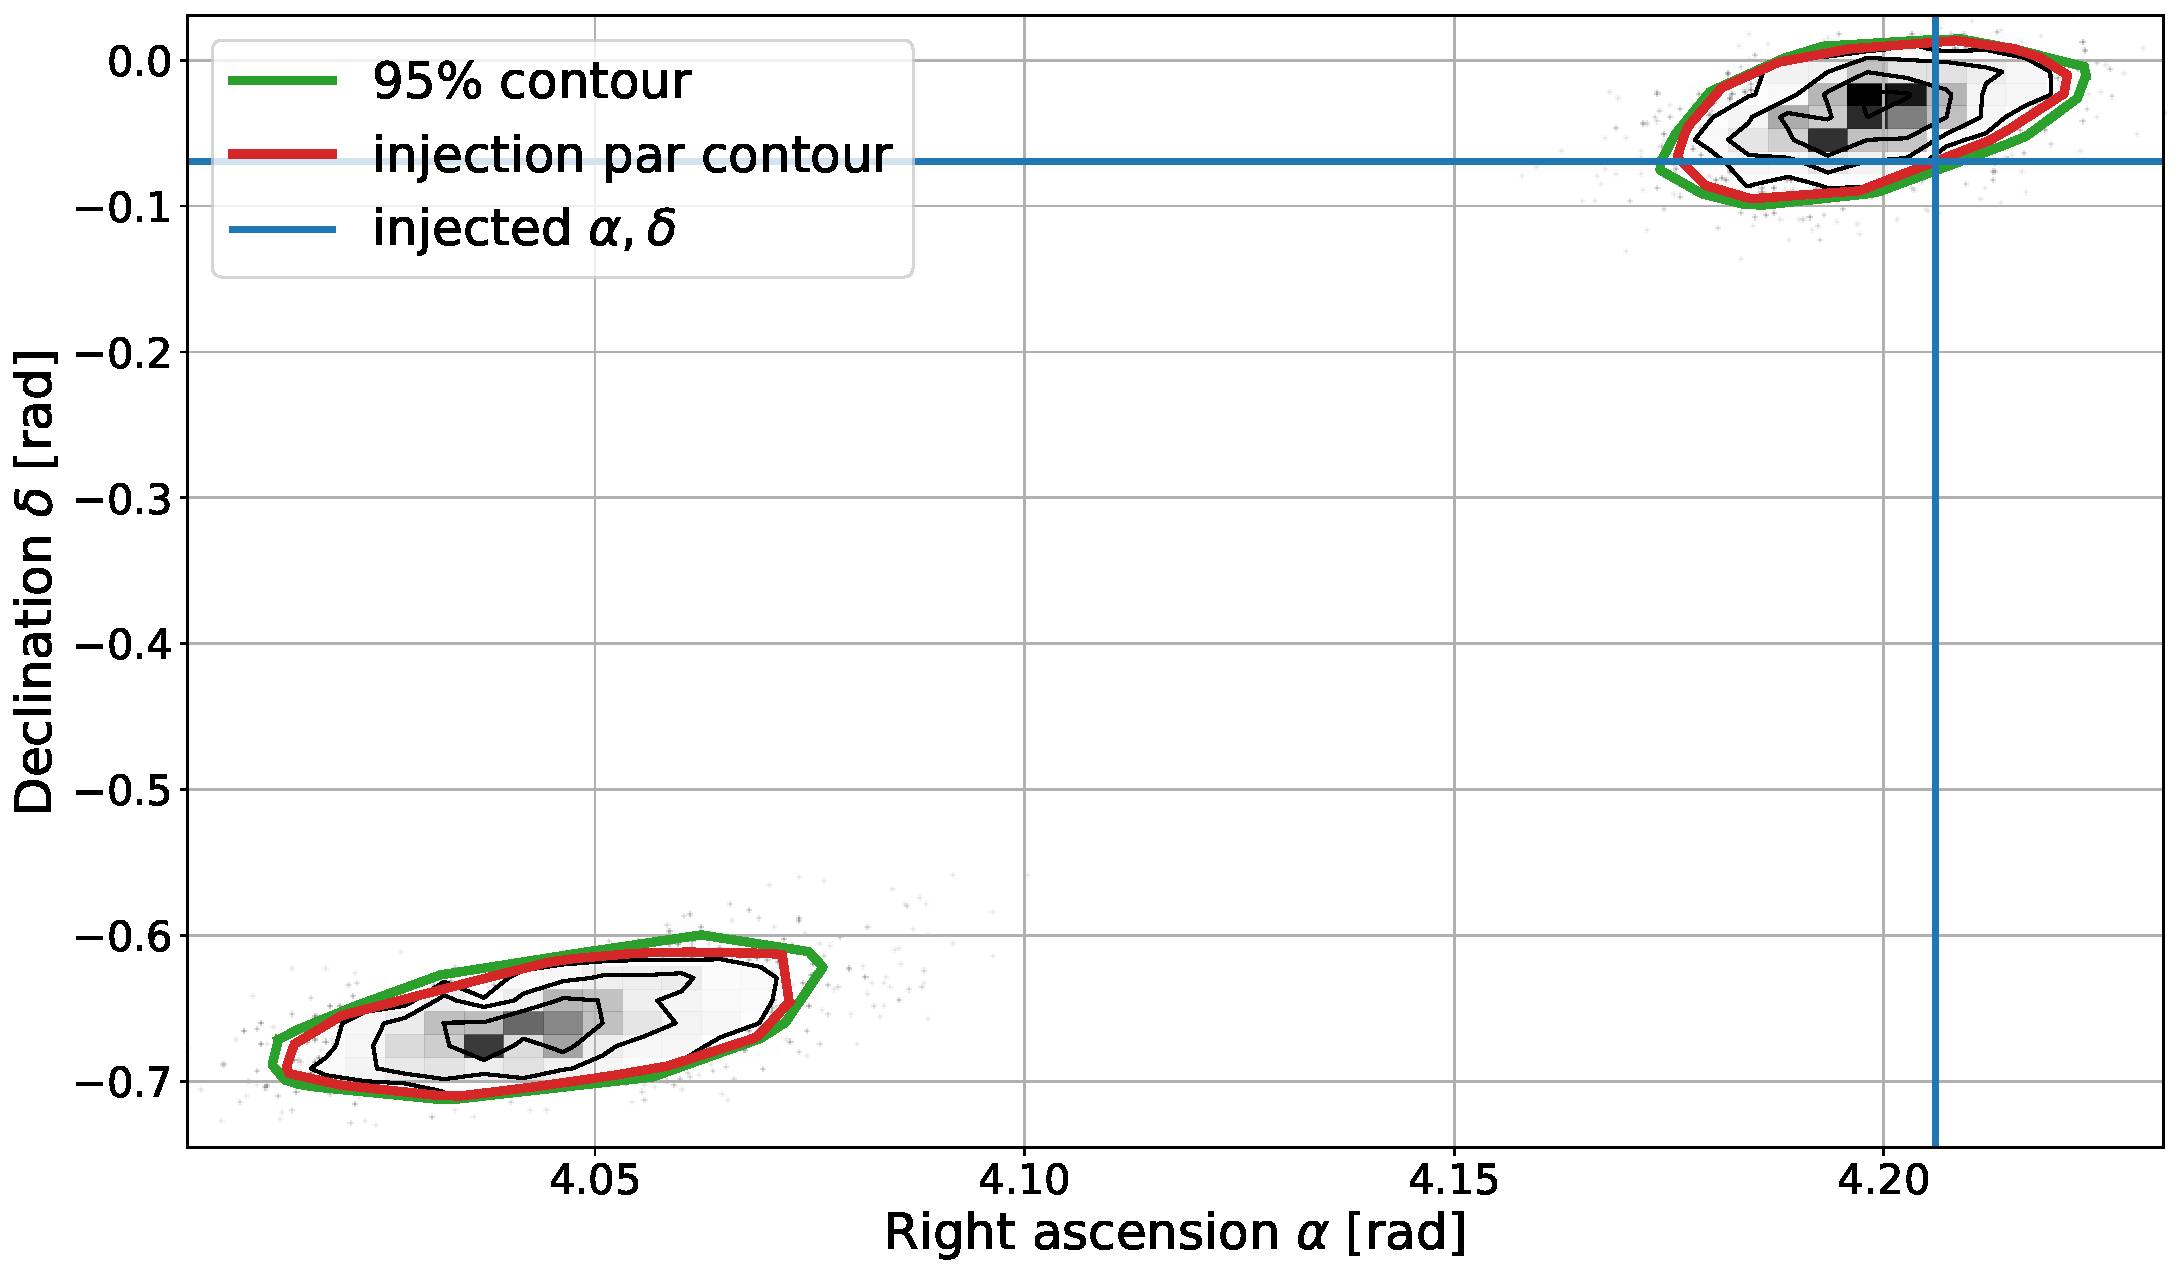
\includegraphics[width=\linewidth]{C5_parameter/skyarea_example.pdf}
    \caption[Area of sky at 95\% confidence]{For the injection in Sec.~\ref{par_est:results:example_posterior}, the contour in sky position posterior is drawn for a 95\% confidence and the area which contains the injected sky position parameters. In this example the two contours are similar.}
    \label{par_est:results:sky_area_example}
\end{figure}

The contours and therefore their associated sky areas can be calculated for all of the simulations described in Sec.~\ref{par_est:results}. 
Figure \ref{par_est:results:sky_area} shows the histograms of the sky areas at 95\% confidence and sky areas which contain the injected parameters.
%
\begin{figure}[ht]
    \centering
    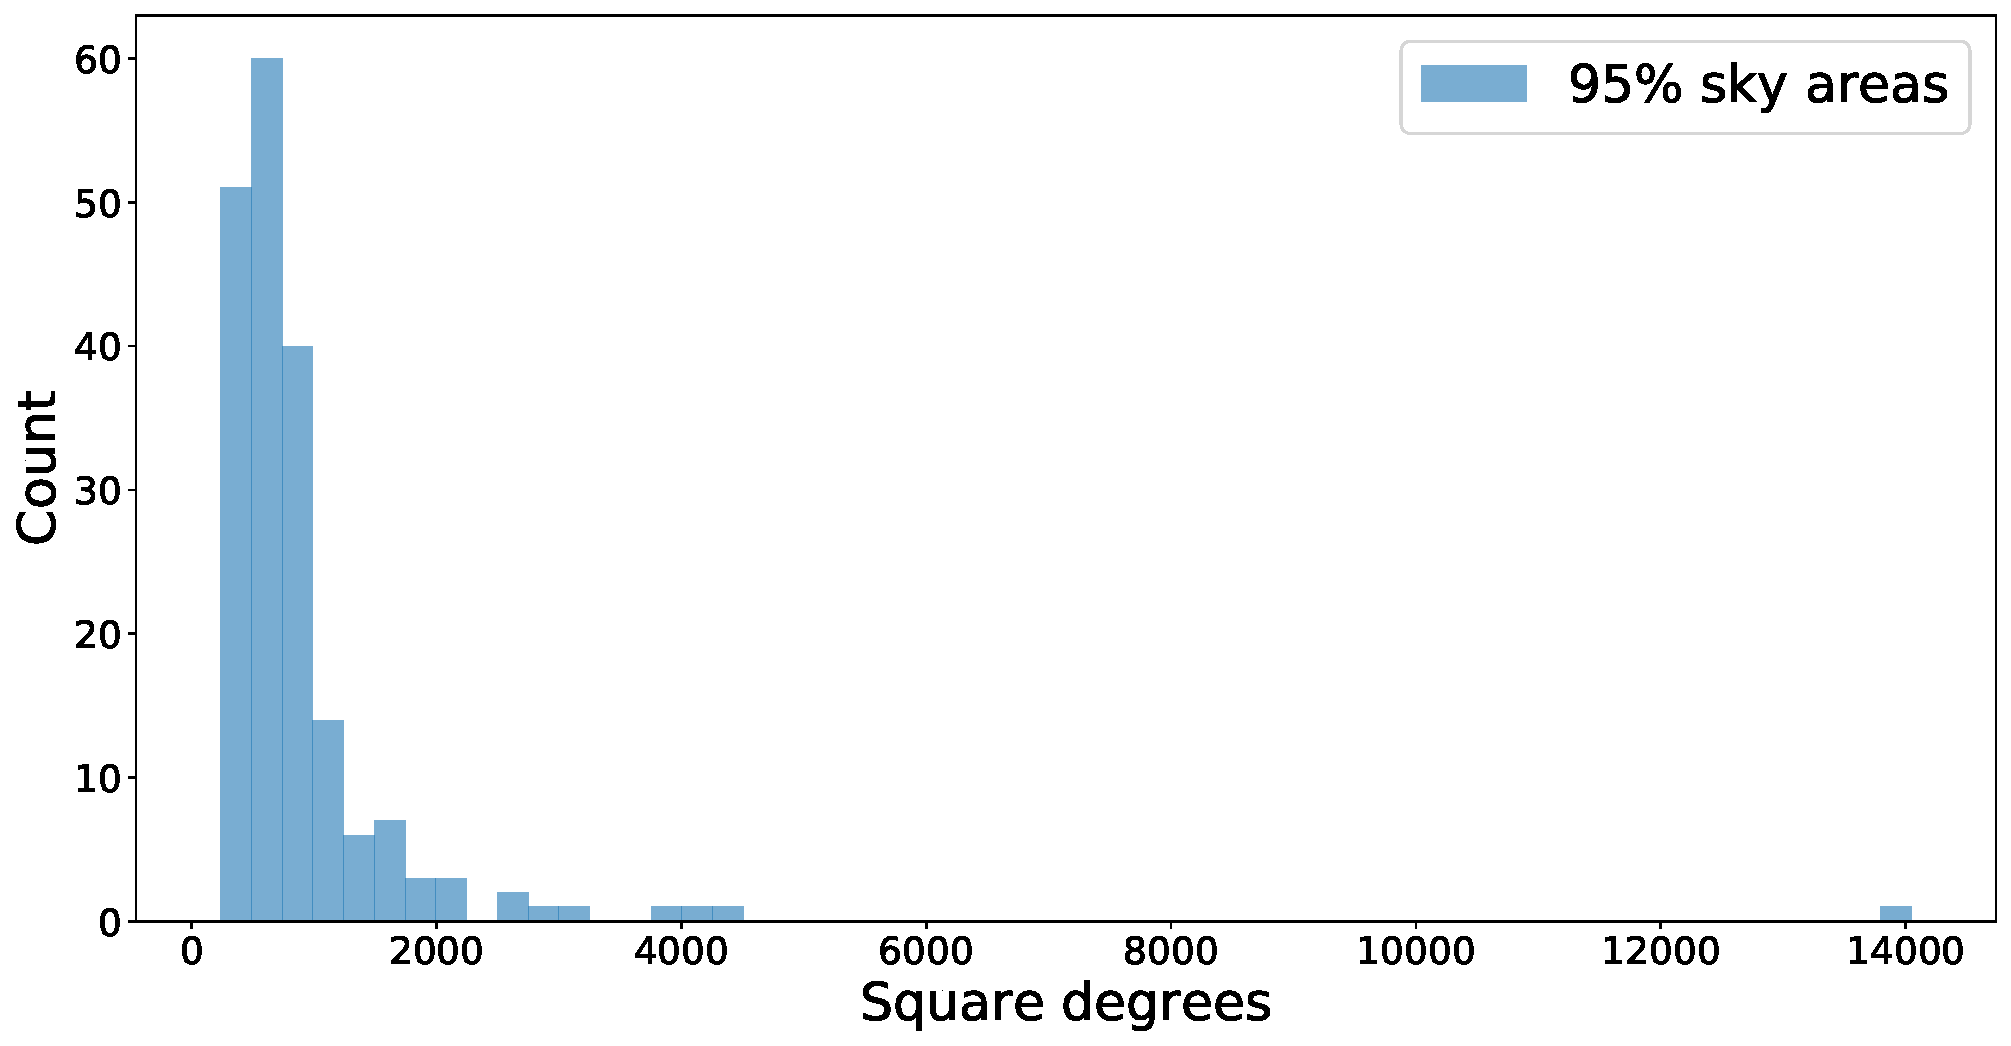
\includegraphics[width=\linewidth]{C5_parameter/sky_area_hist.pdf}
    \caption[p-p plot for the CW simulations]{A histogram is shown of the sky area which this method can localise a source to with 95\% confidence in square degrees and the sky area associated a contour on the posterior that passes through the injected parameter. The entire sky has $\sim 41253$ square degrees, therefore the sky area at 95\% confidence where 90\% of the sky areas are less than this value is 45 deg$^2$.  }
    \label{par_est:results:sky_area}
\end{figure}
%
From the distributions in Fig.~\ref{par_est:results:sky_area} we can see that the sky areas which contain the injected parameters are larger by a factor of $\sim 10$ than those at 95\% confidence.
From this we see that the injected parameters fall within the 95\% confidence contour only 40\% of the time.
This implies that these posterior distributions are over constrained, and the first panel showing the sky areas at 95\% confidence is overly optimistic. \textbf{}

However, if we assume that the 95\% confidence sky areas are correct, we can take the value of the sky area where 90\% of our simulations have a sky area less than this value, i.e. the 90\% confidence line in Fig.~\ref{par_est:results:sky_area}, this is an area of 45 deg$^2$.
Given the full sky has $\sim 41253$ square degrees, this is factor of $\sim 10^{-3}$ of the whole sky.
For an all sky search such as Einstein@Home \citep{theligoscientificcollaborationandthevirgocollaboration2013EinsteinHome,singh2016ResultsAllsky}, which uses the Hough transform \citep{krishnan2004HoughTransform} to combine the coherently analysed segments, the analysis is run at discrete points in parameter space. The initial stage of the search places these points on a coarse grid in sky positions, frequency and frequency derivative to reduce the computational cost.
 If we assume that both the SOAP with parameter estimation method is valid and replaces the first stage in this search, Einstein@Home would only have to search over a factor of $\sim 10^{-3}$ of the sky. 
 Given that this method is $\mathcal{O}(10^4)$ faster than Einstein@home, this would drastically reduce the computational cost of the first stage of the search. 



%
%
\section{Discussion}
%
%

In this chapter I describe a Bayesian analysis to extract the Doppler parameters $\alpha, \delta, f \dot{f}$ and \gls{SNR} $\rho$ of a potential \gls{CW} source from the Viterbi track which is output from the SOAP search in chapter \ref{soap}.
The aim of this method is to provide estimates of the \gls{CW} parameters, and then use these to reduce the size of the parameter space for a more sensitive analysis such as Einstein@Home \citep{singh2016ResultsAllsky}. 

In Sec.~\ref{par_est:bayes} the setup of the Bayesian network is described, where the input is a Viterbi track which is described in chapter \ref{soap}, and the output is a posterior distribution of the Doppler parameters of a \gls{CW} signal.
In this model, the likelihood is empirically calculated by simulating $\mathcal{O}(10^4)$ \gls{CW} signals and then recording the difference between the Viterbi track and \gls{CW} frequency track for multiple \gls{SNR} bands. 
The histogram of these values is then the likelihood of this method.
For each of the parameters in the search, we assume a flat prior.
In Sec.~\ref{par_est:results}, the analysis is tested on 200 simulations which had parameters drawn from the same prior as the Bayesian model.
In this section we generate p-p plots to asses the validity of this model and find that the \gls{SNR}, frequency and frequency derivative all are over constrained distributions and the sky position parameters are under constrained.
However, when looking at the sky position parameters more carefully, we find that the distribution is bi modal where each mode is over constrained.

We investigated the area contained within contours on the marginal posterior for the sky position to gauge the ability of the search to localise a source, where we found that with a 95\% confidence we can detect to a sky area within 45 deg$^2$ 90\% of the time. 
However, due to the over constrained posterior, the true value of the parameter fell within this contour only 40\% of the time.

These results imply that in its current state, the search does not provide a valid way to estimate the parameters of the source from its Viterbi track.
However, with the development of a more appropriate likelihood function and further investigation, we aim to develop this such that it can correctly estimate \gls{CW} parameters.



















